\input{../preamble}
\input{../usercommands}

\begin{document}

\vspace*{2cm}

{\centerline{\bf\huge AST2000 Lecture Notes}}

\vspace*{1cm}

\newcommand{\PartName}{2A}
\newcommand{\refproblem}[1]{\PartName.\ref{#1}}


{\centerline{\bf\LARGE Part \PartName}}\vspace*{0.25cm}
{\centerline{\bf\LARGE The special theory of relativity: Basic principles }}

\vspace*{1cm}

{\centerline{\underline{\LARGE Questions to ponder before the lecture}}}

\vspace*{1cm}

{\large
\begin{enumerate}
\item You have already used the Lorentz transformations. Do you know where they come from? Which basic principles/formulas would you use if you wanted to deduce the Lorentz transformation?
\item You may have heard about the twin paradox: one of the twins is launched into space, travels with a speed close to the speed of light and returns to the Earth. After returning, which of the twins are older?
\item You have already learned how time goes slower when travelling close to the speed of light. So in principle, it is not a paradox that the two twins have different ages after the space trip. What is then the paradox of the twin paradox?
\end{enumerate}

\begin{Figure}%[htb]
\centering
%\begin{center}
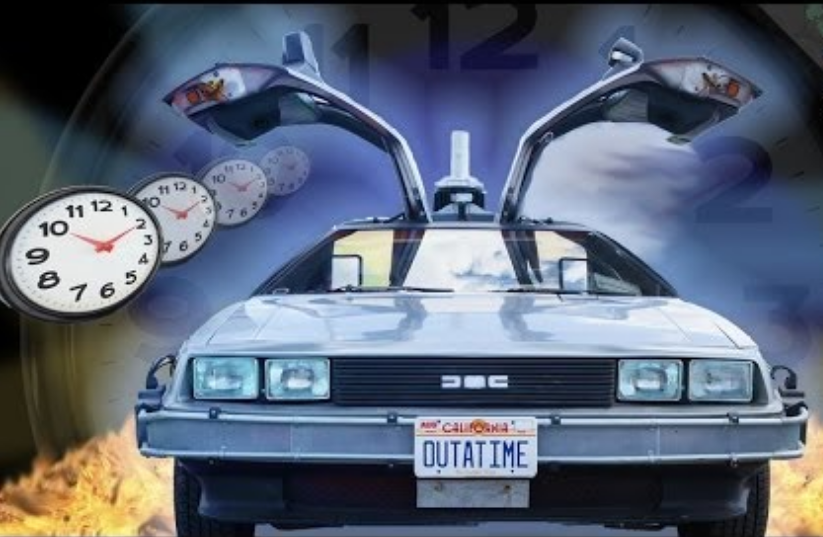
\includegraphics[width=0.8\textwidth]{back_to_the_future.png}
%\end{center}
\end{Figure}
%Image: https://sites.google.com/a/mymodtown.com/imported-site/learn-something-new-videos/What-Back-To-The-Future-Got-Right-About-2015


\clearpage

\vspace*{2cm}

{\centerline{\bf\huge AST2000 Lecture Notes}}

\vspace*{1cm}

{\centerline{\bf\LARGE Part \PartName}}\vspace*{0.25cm}
{\centerline{\bf\LARGE The special theory of relativity: Basic principles }}

\begin{multicols}{2}

\section{Simultaneity}
\label{sect:simul}

We all know that 'velocity' is a relative term. When you specify velocity you need to specify velocity \emph{with respect to something}. If you sit in your car which is not moving (with respect to the ground) you say that your velocity is zero with respect to the ground. But with respect to the Sun you are moving at a speed of $30$~km/s. From the point of view of an observer passing you in his car with a velocity of $100$~km/h with respect to the ground, your speed is $-100$~km/h (see figure \ref{fig:cars}). Even though you are not moving with respect to the ground, you are moving backwards at a speed of $100$~km/h with respect to the passing car. 

In the following we will use the expression \emph{'frame of reference'} to denote a system of observers having a common velocity. All observers in the same frame of reference have zero velocity with respect to each other. An observer always has velocity zero with respect to his own frame of reference. 

An observer on the ground measures the velocity of the passing car to be $100$~km/h with respect to his frame of reference. On the other hand, the driver of the car measures the velocity of the ground to be moving at $-100$~km/h with respect to his frame of reference. 
We will also use the term \emph{'rest frame'} to denote the frame of reference in which a given object has zero velocity. In our example we might say: In the rest frame of the passing car, the ground is moving backwards with $100$~km/h.

\begin{Figure}%[tbp]
%\begin{center}
\centering
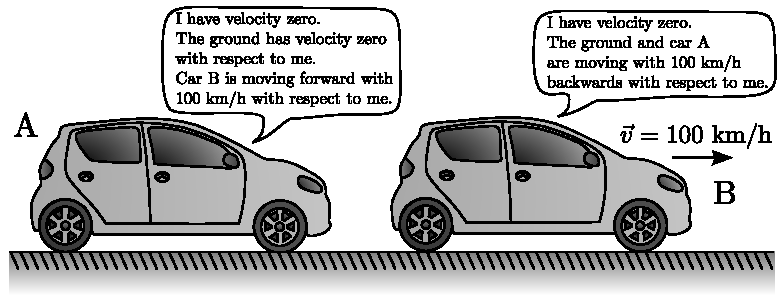
\includegraphics[width=\textwidth]{fig_7-1.pdf}
\captionof{figure}{Velocities are relative.\label{fig:cars}}
%\end{center}
\end{Figure}

You are observing a truck coming towards you with a speed of $v_\mathrm{truck}^\mathrm{ground}=-50$ km/h with respect to the ground (see figure \ref{fig:truck}, velocities are defined to be positive to the right in the figure). From your frame of reference, which is the same frame of reference as the ground, the speed of the truck is $|v_\mathrm{truck}^\mathrm{ground}|=50$ km/h towards you. Now you start driving your car in the direction of the truck with a speed of $v_\mathrm{car}^\mathrm{ground}=+50$ km/h with respect to the ground (see again figure \ref{fig:truck}). From your frame of reference you observe the ground to be moving backwards with a velocity of $v_\mathrm{ground}^\mathrm{car}=-50$ km/h. Again, from your frame of reference you now observe the velocity of the approaching truck to be $v_\mathrm{truck}^\mathrm{car}=v_\mathrm{truck}^\mathrm{ground}-v_\mathrm{car}^\mathrm{ground}=(-50{\rm \ km/h})-(50{\rm \ km/h})=-100{\rm \ km/h}$ (whereas from the frame of reference of an observer on the ground, the truck still has $v_\mathrm{truck}^\mathrm{ground}=-50{\rm \ km/h}$). Now you make a turn so that you drive in the opposite direction: Now your velocity is $-50{\rm \ km/h}$ with respect to the ground, but now you are driving in the same direction as the truck. You are now moving in the same direction as the truck with exactly the same speed with respect to the ground. From your frame of reference (which is now the same frame of reference as the truck) the truck is not moving.

So far, so good. This was just stating some obvious facts from everyday life in a difficult way. Now, replace the truck with a beam of light (a photon) and the car with the Earth. The situation is depicted in figure \ref{fig:mm}. You observe the speed of light from a distant star at two instants: One at the 1st of January, another at the 1st of July. In January you are moving away from the photons approaching you from the distant star. In July you are moving towards the photons arriving from the star. If the speed of light with respect to the distant star is $c$, then in January you expect to measure the speed of the light beam from the star to be $c-v$ where $v=30$ km/h is the speed of the Earth with respect to the same star (we assume that the star does not move with respect to the Sun, so this is also the orbital speed of the Earth). In July you expect to measure the speed of light from the star to be $c+v$, just as for the truck in the example above: The speed of the light beam seen from your frame of reference is supposed to be different depending on whether you move towards it or away from it.

\begin{Figure}%[tpb]
%\begin{center}
\centering
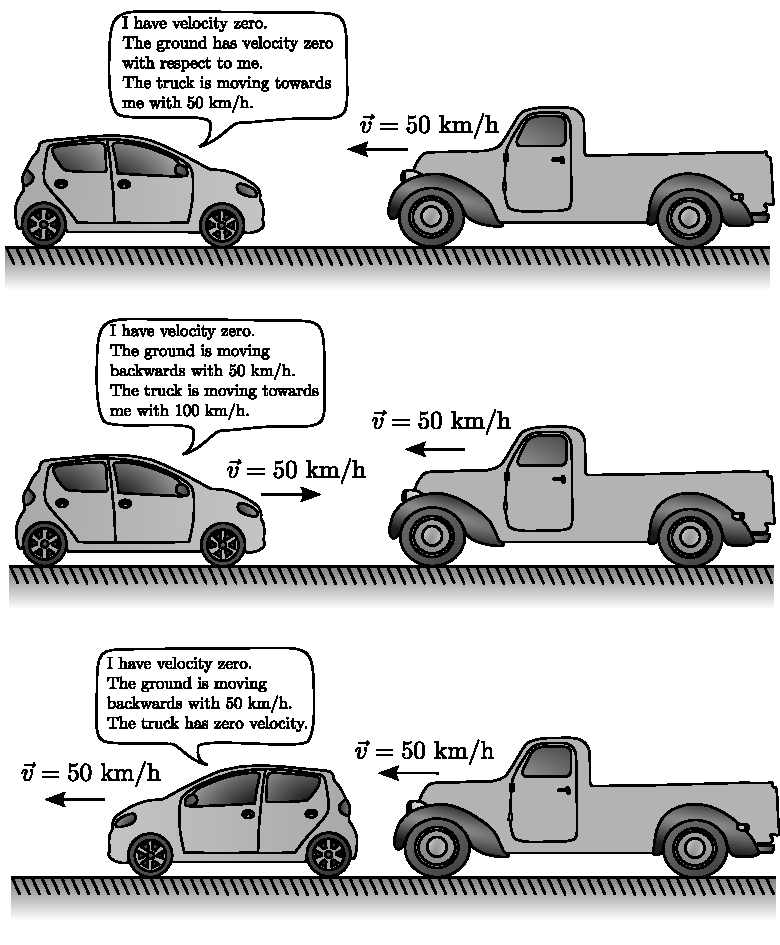
\includegraphics[width=\textwidth]{fig_7-2.pdf}
\captionof{figure}{The velocity of the truck seen from the car depends on the velocity of the car.\label{fig:truck}}
%\end{center}
\end{Figure}

In 1887 Michelson and Morley performed exactly this experiment which is now famous as the 'Michelson-Morley experiment'. The result however, was highly surprising: They measured exactly the same speed of light in both cases. The speed of light seemed to be the same independently of the frame of reference in which it is measured. This has some quite absurd consequences: Imagine that you see the truck driving at the speed of light (or very close to the speed of light, no material particle can ever travel at the speed of light). You are accelerating your car, trying to pass the truck. But no matter at which speed you drive, you see the truck moving with the speed of light with respect to your frame. Even when you reach half the speed of light, you still see the truck moving with velocity $c$. But how is this possible? An observer at rest with respect to the ground measures the truck moving with the speed of light as well, not with the velocity $c+c/2=3c/2$ as you would expect given that it moves with velocity $c$ with respect to something moving with velocity $c/2$.

\begin{Figure}%[tpb]
\centering
%\begin{center}
%\leavevmode
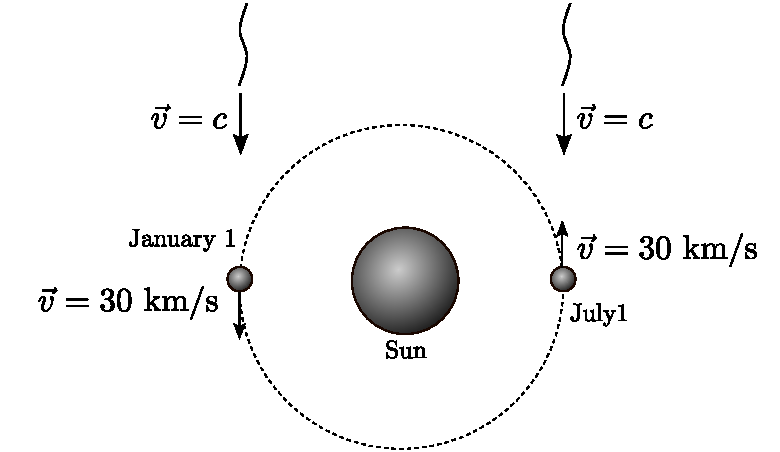
\includegraphics[width=\textwidth]{fig_7-3.pdf}
\captionof{figure}{The velocity of the starlight is measured when the Earth has velocity 30 km/s towards and away from the light beam.\label{fig:mm}}
%\end{center}
\end{Figure}

\begin{Figure}%[tpb]
%\begin{center}
\centering
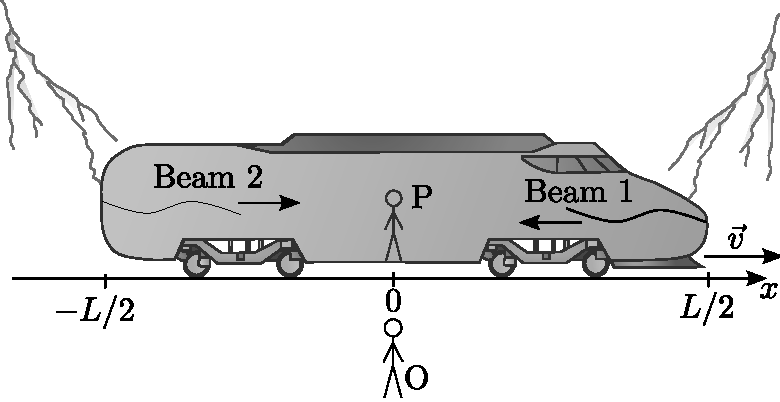
\includegraphics[width=\textwidth]{fig_7-4x.pdf}
\captionof{figure}{Event A: Lightning strikes the front part of the train. Event B: Lightning strikes the rear part of the train. These two events are observed by observer O on the ground and observer P in the train. The train has length L.\label{fig:train}}
%\end{center}
\end{Figure}

This was one of the first signs showing that something was wrong with classical physics. The fact that the speed of light seemed to be constant in all frames of reference led to several contradictions. We have already seen one example of such a contradiction. We will now look at another one which might shed some light on the underlying reason for these contradictions. 

In figure \ref{fig:train} we show the situation. Observer O is standing on the ground (at rest with respect to the ground), observer P is standing in the middle of a train of length $L$ moving with velocity $v$ with respect to the ground. Observer O sees two lightnings striking the front and the rear of the train simultaneously. We call the two events A and B (An event is a point in space and time, a point with a space and time coordinate): Event A is the lightning striking the front, event B is the lightning striking the rear. Events A and B are simultaneous. 

The light from these two lightnings start traveling from the front and back end of the train towards observer P. The beam approaching observer P from the front is called beam 1 and the beam approaching from the rear is called beam 2. 

Both observers had synchronized their clocks to $t=0$ at the instant when the lightnings strike the train. Both observers have also defined their own coordinate systems $x$ (observer on the ground) and $x'$ (observer in the train) which is such that the position of observer P is at $x=x'=0$ in both coordinate systems at the instant $t=0$ when the lightenings strike. Thus the lightnings hit the train at the points $x=x'=L/2$ and $x=x'=-L/2$ as seen from both observers. We will now look how each of these observers experience these events:

{\bf From the point of view of observer O standing on the ground:}

The frame of reference of observer O on the ground is often referred to as the {\it laboratory frame \label{pg:labframe}}. It is the frame of reference which we consider to be at rest. At what time $t=t_C$ does observer P see beam 1 (we call this event C)? To answer this question, we need to have an expression for the x-coordinate of observer $P$ and the x-coordinate of beam 1 at a given time $t$. Observer P moves with constant velocity $v$ so his position at time $t$ is $x_P=vt$. Beam 1 moves in the negative x-direction with the speed of light $c$ starting from $x_1=L/2$ at $t=0$. The expression thus becomes $x_1=L/2-ct$. Observer P sees beam 1 when $x_1=x_P$ at time $t_C$. Equating these two expressions, we find
\begin{equation}
\label{eq:tc}
t_C=\frac{L/2}{c+v}.
\end{equation}

At what time $t=t_D$ does observer P see beam 2 (we call this event D)? Following exactly the same line of thought as above, we find
\begin{equation}
\label{eq:td}
t_D=\frac{L/2}{c-v}.
\end{equation}
So according to observer O in the laboratory frame, $t_C<t_D$ and observer P should see the light beam from the lightning in front before the light from the back. This sounds reasonable: Observer P is moving towards beam 1 and away from beam 2 and should therefore see beam 1 first.

{\bf From the point of view of observer P standing in the train:}

At what time $t=t_C$ does observer P see beam 1? We have just agreed on the fact that the speed of light is independent of the frame of reference. The result is that the speed of light is $c$ also for the observer in the train. Seen from the frame of reference of observer P, observer P himself is at rest and the ground is moving backwards with speed $v$. Thus from this frame of reference, observer P is always standing at the origin $x_P'=0$ (the coordinate system $x'$ moves with observer P). The expression for $x_1'$ is the same as seen from observer O:$x_1'=L/2-ct$ (convince yourself that this is the case!). Again we need to set $x_1'=x_P'$ giving
\[
t_C=\frac{L/2}{c}
\]

At what time $t=t_D$ does observer P see beam 2? Again we follow the same procedure and obtain
\[
t_D=\frac{L/2}{c}
\]
As calculated from the frame of reference of observer P, the two beams hit observer P at exactly the same time.

So not only are the exact times $t_C$ and $t_D$ different as calculated from the two frames of reference, but there is also an even stronger contradiction: Observer P should be hit by the two beams simultaneously as calculated from the frame of reference of observer P himself, but as calculated from the laboratory frame, beam 1 hits observer P before beam 2. What does really happen? Do the beams hit observer P simultaneously or not? Well, let's ask observer P himself:

{\sf So observer P, two lightnings struck your train simultaneously at the front and rear end. Did you see these two lightnings simultaneously or did you see one flash before the other?}\\
{\sf Observer P: Sorry? I think you are not well informed. The two lightnings did not happen simultaneously. There was one lightning which struck the front part and then shortly afterwards there was another one striking the rear. So clearly I saw the flash in the front first.}\\
{\sf Observer O: No, no, listen, the lightnings did strike the train simultaneously, there was no doubt about that. But you were moving in the direction of beam 1 and therefore it appeared to you that the front was hit by the lightning first.}\\
{\sf Observer P: So you didn't watch very carefully I see. It is impossible that the two lightnings struck at the same time. Look, I was standing exactly in the middle of the train. The speed of light is always the same, no matter from which direction it arrives. Beam 1 and beam 2 had to travel exactly the same distance $L/2$ with exactly the same speed $c$. If the beams were emitted simultaneously I MUST have seen the two flashes at the same time. But I didn't....beam 1 arrived before beam2, and so event A must have happened before event B}

So beam 1 did indeed hit observer P before beam 2. And indeed, observer P has got a point: From observer P the two lightnings could not have occurred at the same time. Asking observer O one more time he says that he is absolutely certain that the two lightnings struck simultaneously. Who is right?

We have arrived at one of the main conclusions that Einstein reached when he was discovering the theory of relativity: \emph{simultaneity is relative}. If two events happen at the same time or not depends on who you ask. It depends on your frame of reference. In the example above, the two lightnings were simultaneous for the observer at rest on the ground, but not for the observer moving with velocity $v$. This has nothing to do with the movement of the light beams, it is simply time itself which is different as seen from two different frames of reference. Simultaneity is a relative term in exactly the same way as velocity is: When you say that two events are simultaneous you need to specify that they are simultaneous with respect to some frame of reference.

In order to arrive at the conclusion of the relativity of simultaneity, Einstein excluded an alternative: Couldn't it be that the laws of physics are different in different frames of reference? If the laws of physics in the train were different from those in the laboratory frame, then simultaneity could still be absolute. The problem then is that we need to ask the question 'Physics is different in frames which move with respect to {\it which} frame of reference?'. In order to ask this question, velocity would need to be absolute. If velocity is relative, then we can just exchange the roles: The observer in the train is at rest and the observer on the ground is moving. Then we would need to change the laws of physics for the observer on the ground. This would lead to contradictions. In order to arrive at the theory of relativity, Einstein postulated the {\it Principle of Relativity \label{pg:por}}. The principle of relativity states that all laws of physics, both the mathematical form of these laws as well as the physical constants, are the same in all {\it free float frames\label{pg:ff}}. In the lectures on general relativity we will come back to a more precise definition of the free float frame. For the moment we will take a free float frame to be a frame which is not accelerated, i.e.\ a frame in which we do not experience fictive forces. You can deduce the laws of physics in one free float frame and apply these in any other free float frame. Imagine two space ships, one is moving with the velocity $v=1/2c$ with respect to the other. If you close all windows in these spaceship there is no way, by performing experiments inside these spaceships, that you can tell which is which. All free float frames are equivalent, there is no way to tell which one is at rest and which one is moving. Each observer in a free float frame can define himself to be at rest.

 

\section{Invariance of the spacetime interval}
\label{sect:invariance}

We have seen that two events which are simultaneous in one frame of reference are not simultaneous in another frame. We may conclude that time itself is relative. In the same way as we needed two coordinate systems $x$ and $x'$ to specify the position in space relative to two different frames, we need two time coordinates $t$ and $t'$ to specify the time of an event as seen from two different frames. We are used to think of time as a quantity which has the same value for all observers but we now realize that each frame of reference has its own measure of time. Clocks are not running at the same pace in all frames of reference. Observers which are moving with respect to each other will measure different time intervals between the same events. Time is not absolute and for this reason simultaneity is not absolute.

\begin{Figure}%[tpb]
%\begin{center}
\centering
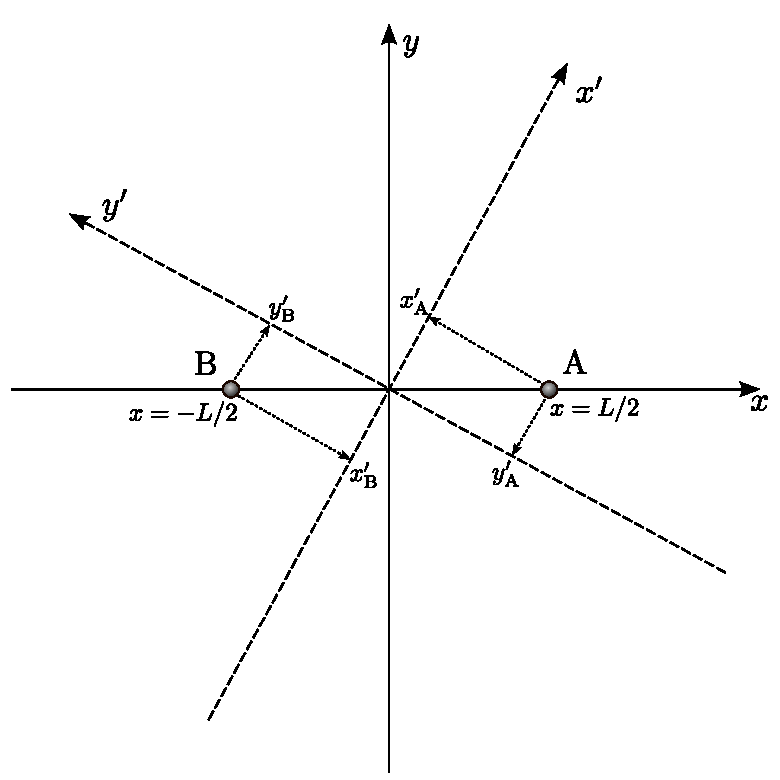
\includegraphics[width=\textwidth]{fig_7-5.pdf}
\captionof{figure}{The position of two points A and B measured in two different coordinate systems rotated with respect to each other.\label{fig:xy}}
%\end{center}
\end{Figure}

Look at figure \ref{fig:xy}. It shows two points $A$ and $B$ and two coordinate systems $(x,y)$ and $(x',y')$ rotated with respect to each other. The two points A and B are situated at a distance $\Delta x_{AB}=L$ and at the same y-coordinate $\Delta y_{AB}=0$ in the $(x,y)$ system. In the rotated $(x',y')$ system however, there is a non-zero difference in the y-coordinate, $\Delta y_{AB}\ne0$. Now, replace $y$ with $t$. Do you see the analogy with the example of the train above?

If we replace $y$ with $t$ and $y'$ with $t'$, then the two points A and B are the events A and B in {\it spacetime}. Our diagram is now a {\it spacetime diagram\label{pg:spacetimediag}} showing the position of events in space $x$ and time $t$, rather than a coordinate system showing the position of a point in space $(x,y)$. Consider the two coordinate systems $(x,t)$ and $(x',t')$ as measurements in two different frames of reference, the lab frame and the frame of observer P. We see that in the $(x,t)$ system, the two events are simultaneous $\Delta t_{AB}=0$ whereas in the $(x',t')$ system, the events take place at two different points in time.

We are now entering deep into the heart of the special theory of relativity: We need to consider time as the {\it fourth dimension}. And moreover, we need to treat this fourth dimension similar (but not identical) to the three spatial dimensions. That is, we need to talk about distances in space and distances in time. But, you might object, we measure distances in space in meters and time intervals in seconds. Can they really be similar? Yes they can, and you will soon get rid of the bad habit of measuring space and time in different units. From now on you will either measure both space \emph{and} time in meters, or both time \emph{and} space in seconds. By the time you have finished this course you will, without thinking about it, ask the lecturer how many meters the exam lasts or complain to your friends about how small your room in the dormitory is, giving them the size in square seconds.

How do you convert from meters to seconds and vice versa? The conversion factor is given by the universal factor $c$, the speed of light. If you have a time interval measured in seconds, multiply it by $c$ and you have the time interval in meters. If you have a distance in space measured in meters, divide it by $c$ and you obtain the distance measured in seconds:
\[
x=ct,\ \ \ t=x/c.
\]
From now on we will drop the factor $c$ and suppose that distances in space and time are measured in the same units. When you put numbers in your equations you need to take care that you always add quantities with the same units, if you need to add two quantities with different units, the conversion factor is always a power of $c$.

Measuring time in meters might seem strange, but physically you can think about it this way: Since the conversion factor is the speed of light, a time interval measured in meters is simply the distance that light travels in the given time interval. If the time interval between two events is 2 meters, it means that the time interval between these events equals the time it takes for light to travel 2 meters. We might say that the time interval between these events is 2 meters of light travel time. Similarly for measuring distances in seconds: If the spatial distance between two events is 10 seconds, it means that the distance equals the distance that light travels in 10 seconds. The distance is 10 light seconds. Actually you are already accustomed to measure distances in time units: You say that a star is 4 light years away, meaning that the distance equals the distance that light travels in four years. Note also one more effect of measuring space and time in the same units: Velocities will be dimensionless. Velocity is simply distance divided by time, if both are measured in meters, velocity becomes dimensionless. We can write this as $v_\mathrm{dimensionless}=dx/(cdt)=v/c$ (to convert $dt$ to units of length we need to multiply it by $c$, thus $cdt$). If the velocity $v=dx/dt=c$ is just the speed of light, we get $v_\mathrm{dimensionless}=1$. From now on we will just write $v$  for $v_\mathrm{dimensionless}$. Note that some books use $\beta$ to denote dimensionless velocity, here we will use $v$ since we will always use dimensionless velocities when working with the theory of relativity. The absolute value of velocity $v$ is now a factor in the range $v=[0,1]$ being the velocity relative to the velocity of light. 

This was the first step in order to understand the foundations of special relativity. Here comes the second: Let us, for a moment, return to the spatial coordinate systems $(x,y)$ and $(x',y')$ in figure \ref{fig:xy}. Clearly the coordinates of the points $A$ and $B$ are different in the two coordinate systems. But there is one thing which is identical in all coordinate systems: The distance between points A and B. If we call this distance $\Delta s_{AB}$ we can write this distance in the two coordinate systems as


\begin{eqnarray*}
(\Delta s_{AB})^2&=&(\Delta x_{AB})^2+(\Delta y_{AB})^2\\
(\Delta s_{AB}')^2&=&(\Delta x_{AB}')^2+(\Delta y_{AB}')^2
\end{eqnarray*}
(check that you understand why!). The distance between A and B has to be equal in the two coordinate systems, so
\[
(\Delta s_{AB})^2=(\Delta s_{AB}')^2.
\]
Is this also the case in spacetime? Can we measure intervals between events in spacetime? This is now, at least in theory, possible since we measure space and time separations in the same units. In a spatial $(x,y,z)$ system we know the geometrical relation,
\[
(\Delta s)^2=(\Delta x)^2+(\Delta y)^2+(\Delta z)^2,
\]
from Euclidean geometry: The square of the distance between two points (called the {\it line element\label{pg:lineelement}}) is simply the sum of the squares of the coordinate distances between these two points. But do the rules of Euclidean geometry apply to spacetime? No, not entirely. The geometry of spacetime is called {\it Lorentz geometry\label{pg:lorentz}}. The distance between two events (line element) in Lorentz spacetime $\Delta s^2$, is given by
\begin{formbox}
\textbf{The spacetime interval}
\[
(\Delta s)^2=(\Delta t)^2-(\Delta x^2+\Delta y^2+\Delta z^2).
\]
\end{formbox}
Note the minus sign. This minus sign is the only thing which distinguishes space from time. The square of the spacetime distance between two events equals the square of the time separation between these events \emph{minus} the square of the spatial separations between the events. And in the same way as the distance between two points in space is the same in all coordinate systems, the distance in spacetime, {\it the spacetime interval\label{pg:spacetimeinterval}} is the same in all frames of reference. We say that the spacetime interval is {\it invariant\label{pg:invariant}}. A quantity is invariant if it has the same value in all frames of reference. We already know another invariant quantity: the speed of light.


So, that was it. We're done. Now you know what the special theory of relativity is all about. Congratulations! You now see that we may write the special theory of relativity in two sentences: Measuring space and time intervals in the same units, you can calculate the spacetime interval between two events using the formula for the line element in Lorentz geometry. This spacetime interval between two events is invariant, it has the same value as measured from all frames of reference. We will now see what this means in practice. But before you continue, take a walk, go for a coffee or simply take half an hour in fresh air. Your brain will need time to get accustomed to this new concept.

\section{An example}
\label{sect:example}

A train is moving along the x-axis of the laboratory frame. The coordinate system of the laboratory frame is $(x,y)$ and of the train, $(x',y')$. In the train a light signal is emitted directly upwards along the y-axis (event A). Three meters above, it is reflected in a mirror (event B) and finally returns to the point where it was emitted (event C). In the train frame it takes the light beam 3 meters of time to reach the mirror and 3 meters of time to return to the point where it was emitted. The total up-down trip (event A to event C) took 6 meters of time in the frame of the train (light travels with a speed of $v=1$, one meter per meter of light travel time). From event A to event C, the train had moved 8 meters along the x-axis in the laboratory frame. Because of the movement of the train, the light beam moved in a pattern as shown in figure \ref{fig:example} seen from the lab frame. 

\begin{Figure}%[tpb]
%\begin{center}
\centering
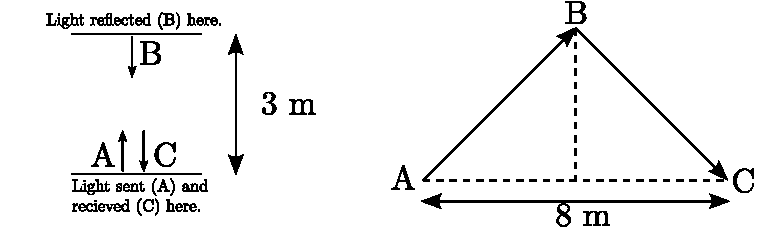
\includegraphics[width=\textwidth]{fig_7-6.pdf}
\captionof{figure}{The light emitted (event A) upwards in the train is reflected (event B) and received (event C) at the same place (in the train frame) as it was emitted.\label{fig:example}}
%\end{center}
\end{Figure}

\begin{enumerate}
\item {\it Use the figure to find the total distance $d$ traveled by the light beam in the laboratory frame.} Dividing the triangle into two smaller triangles (see the figure), we find from one triangle that the distance traveled from the emission of the light beam to the mirror is $d/2=\sqrt{(4{\rm \ m})^2+(3{\rm \ m})^2}=5{\rm \ m}$ and similarly for the return path. Thus, the total distance traveled by the light beam from event A to event C is $d=10{\rm \ m}$.
\item {\it What was the total time it took for the light beam from event A to event C in the laboratory frame?} We have just seen that in the laboratory frame, the light beam traveled 10 meters from event A to event C. Since light travels at the speed of one meter per meter of time, it took 10 meters of time from event A to event C. In the frame of the train, it took only 6 meters of time.
\item {\it What is the speed of the train?} The train moved 8 meters in 10 meters of time, so the speed is $v=8/10=4/5$, 4/5 the speed of light.
\item {\it What is the spacetime interval $\Delta s'$ between event A and event C with respect to the train frame?} In the train frame, event A and event C happened at the same point, so $\Delta x'=0$. It took 6 meters of time from event A to event C, so $\Delta t'=6{\rm \ m}$. The spacetime interval is thus $\Delta s'=\sqrt{(6{\rm \ m})^2-0}=6{\rm \ m}.$ (check that you also got this result!)
\item {\it What is the spacetime interval $\Delta s$ between event A and event C with respect to the laboratory frame?} In the laboratory frame, the distance between the events were $\Delta x=8{\rm \ m}$ and the time interval was $\Delta t=10{\rm \ m}$. The spacetime interval is thus $\Delta s=\sqrt{(10{\rm \ m})^2-(8{\rm \ m})^2}=6{\rm \ m}$ (check that you also got this result!), exactly the same as $\Delta s'$ in the train frame.
\item {\it Was there an easier way to answer the previous question?} Oh\ldots uhm, yes, you're right, the spacetime interval is the same in all frames of reference so I should immediately had answered $\Delta s=\Delta s'=6{\rm \ m}$ without any calculation\ldots  much easier!
\end{enumerate}
Indeed much easier\ldots remember that this will be very useful when calculating distances and intervals with respect to frames moving close to the speed of light.

\begin{figure*}
\fcolorbox{black}{yellow}{\parbox{\dimexpr \linewidth-2\fboxsep-2\fboxrule}{
\begin{minipage}{0.5\textwidth}%{\dimexpr\linewidth-2\fboxsep-2\fboxrule}\parskip=6pt
{\small
\fontfamily{bch}\selectfont
\vspace*{-0.1cm}\hspace*{-0.15cm}\fcolorbox{black}{black}{\bf\color{white} Fact sheet:\color{black}} 
Near the beginning of his career, Albert Einstein (1879–1955) thought that Newtonian mechanics was no longer enough to reconcile the laws of classical mechanics with the laws of the electromagnetic field. This led to the development of his special theory of relativity (1905). It generalizes Galileo's principle of relativity – that all uniform motion is relative, and that there is no absolute and well-defined state of rest – from mechanics to all the laws of physics. Special relativity incorporates the principle that the speed of light is the same for all inertial observers regardless of the state of motion of the source. This theory has a wide range of consequences that have been experimentally verified, including length contraction, time dilation and relativity of simultaneity, contradicting the classical notion that the duration of the time interval between two events is equal for all observers. On the other hand, it introduces the spacetime interval, which is invariant.
}
\end{minipage}%\hspace*{0.5cm}
\ \ \ \ \ \ \begin{minipage}{0.4\textwidth}
\centering
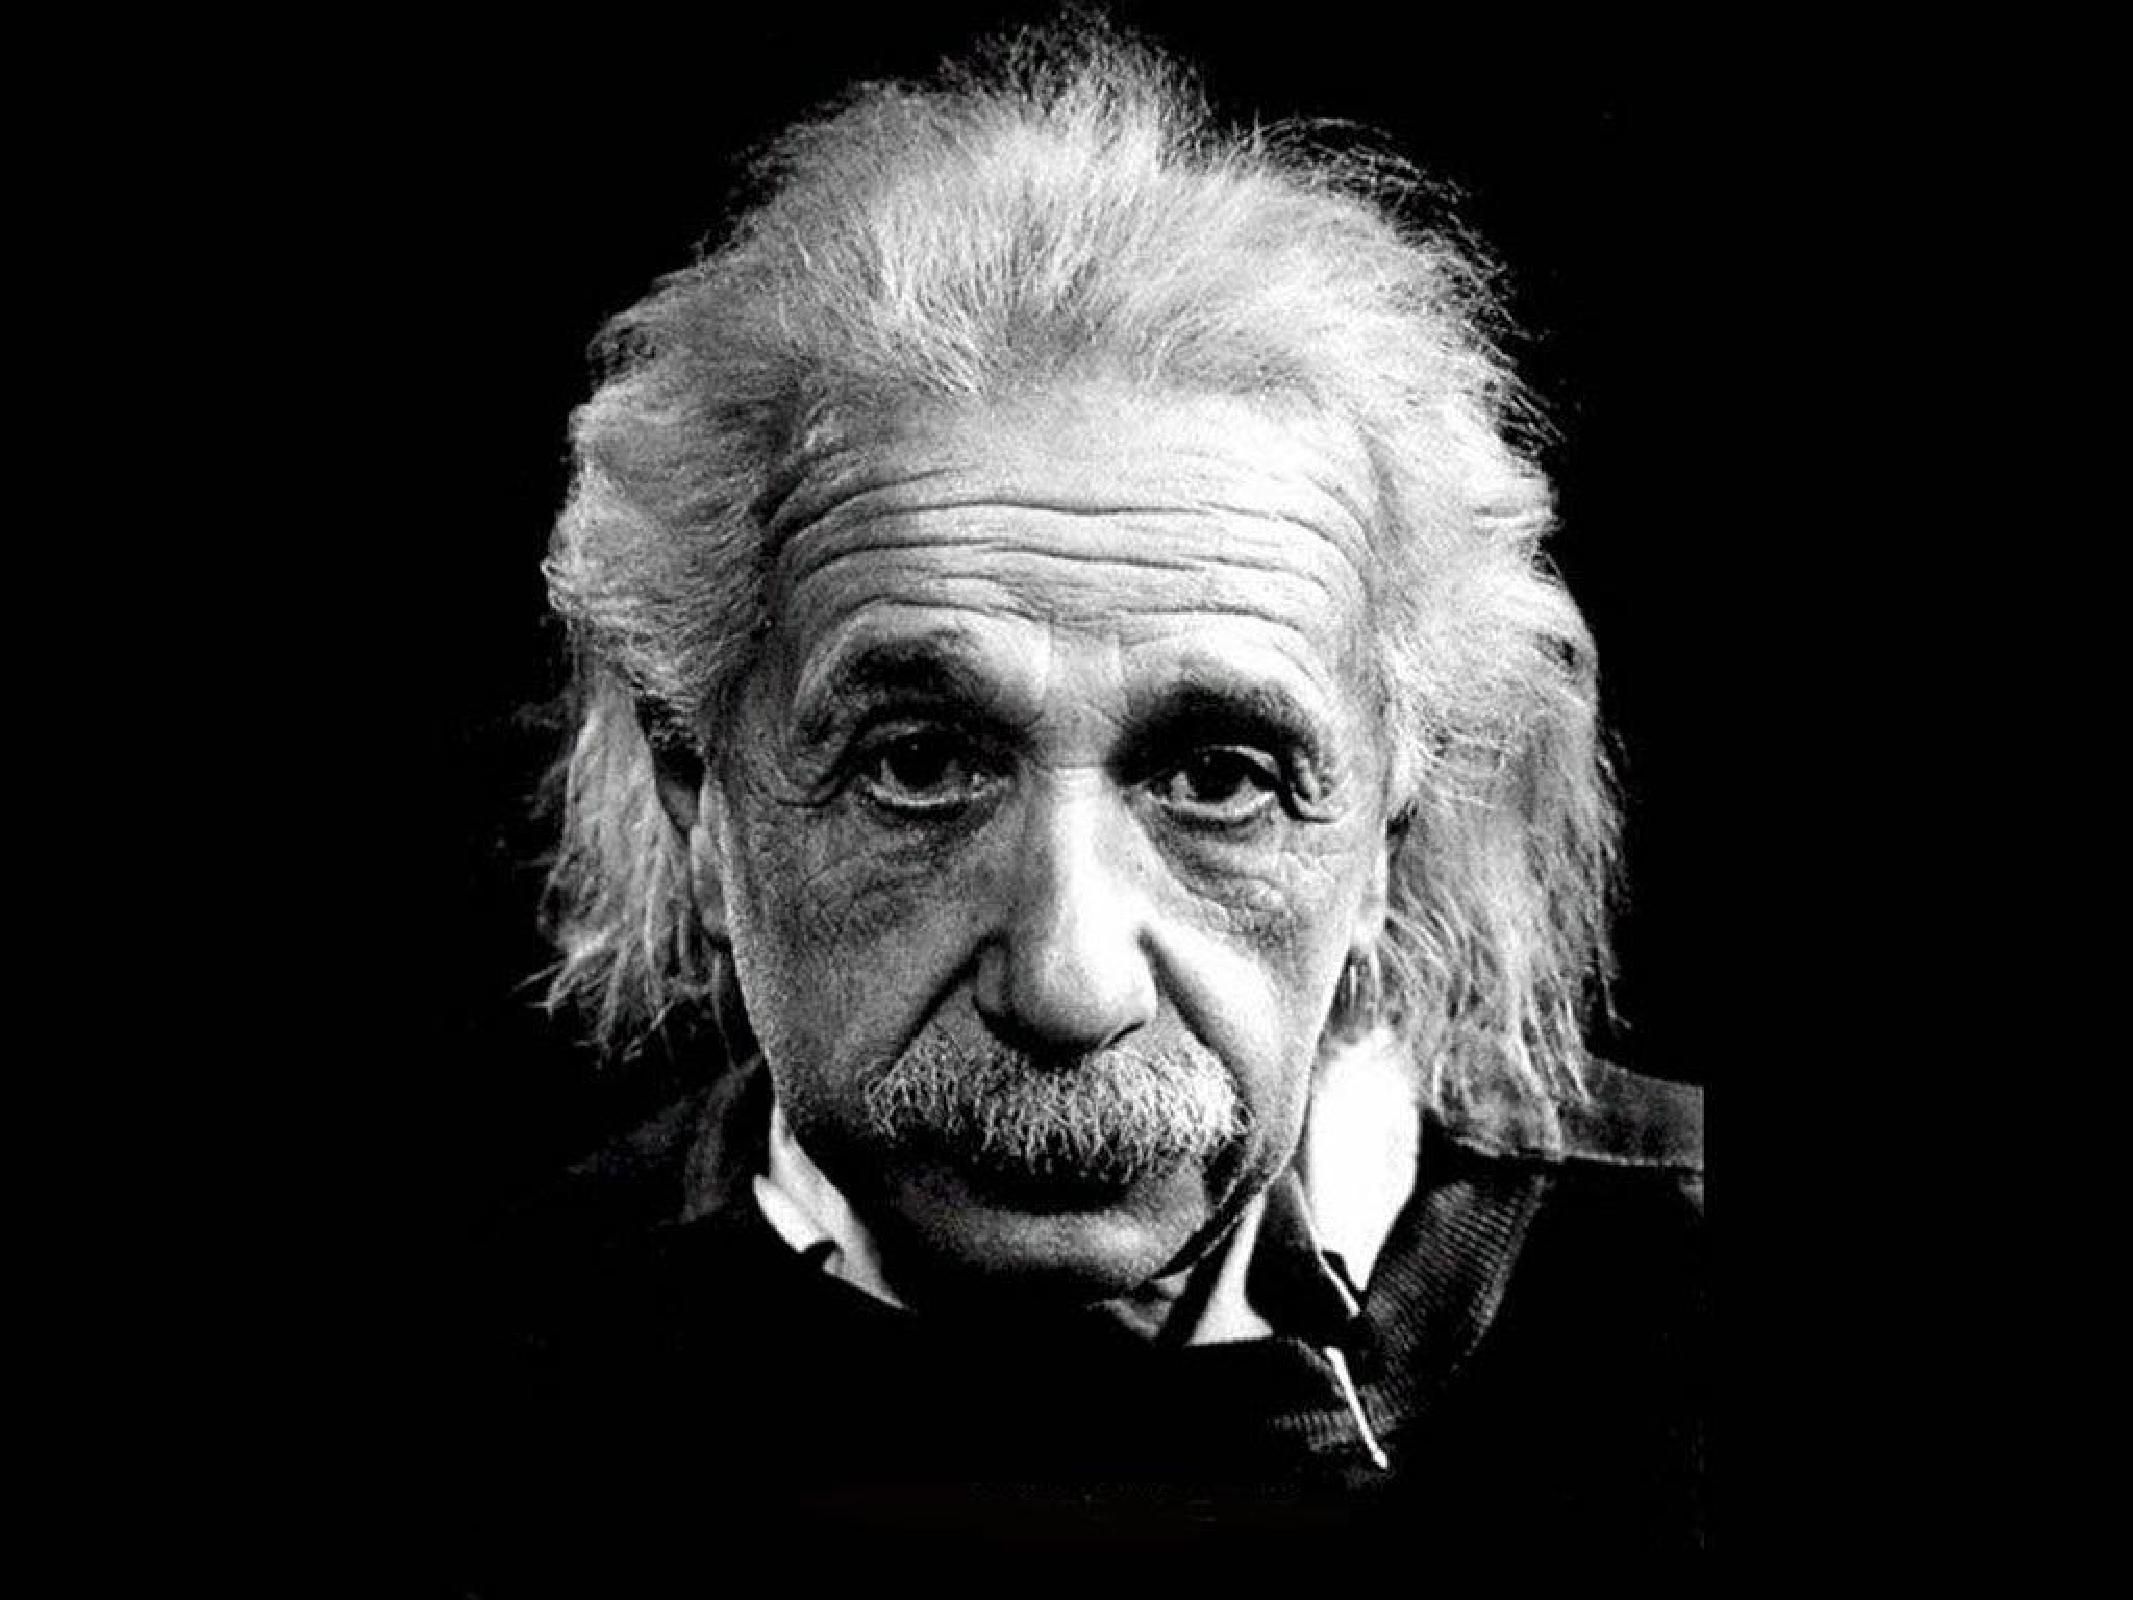
\includegraphics[width=\textwidth,height=0.25\textheight]{Einstein.pdf}
%\end{wrapfigure}
%\end{center}
%\end{figure*}
\end{minipage}
}}
\end{figure*}

\section{Observer O and P revisited}
\label{sect:oandp}

Armed with the knowledge of the invariance of the spacetime interval we now return to observer O and P in order to sort out exactly what happened for each of the observers. We know that with respect to the laboratory frame, the two lightnings struck simultaneously (events A and B were simultaneous) at points $x=\pm L/2$ at the time $t=0$ when observer P was at the origin $x_P=0$. But at what time did the two lightnings strike with respect to observer P in the train? We have learned that with respect to the frame of reference following the train, the events A and B were \emph{not} simultaneous. But in the reference frame of observer P, at what time $t_A'$ and $t_B'$ did the two lightnings strike? The two observers exchange a signal at $t=0$ such that their clocks are both synchronized to $t=t'=0$ at the instant when observer P is at the origin in both coordinate systems $x_P=x_P'=0$. Did event A and B happen before or after $t'=0$ on observer P's wristwatch? (It is common to talk about \emph{wristwatches} when referring to the time measured in the rest frame of a moving object, i.e.\ the time measured by observers moving with the object. This wristwatch time is also called {\it proper time\label{pg:propertime}}).

We know that an event is characterized by a position $x$ and a time $t$ in each of the frames of reference. Let's collect what we know about the position and time of event A, B and the event when observer P passes $x=x'=0$ which we call event P:

{\bf Event P:}
\begin{eqnarray*}
x=0 & t=0\\
x'=0 & t'=0
\end{eqnarray*}

{\bf Event A:}
\begin{eqnarray*}
x=L/2 & t=0\\
x'=L_0/2 & t'=t_A'
\end{eqnarray*}

{\bf Event B:}
\begin{eqnarray*}
x=-L/2 & t=0\\
x'=-L_0/2 & t'=t_B'
\end{eqnarray*}

Note that the length of the train is $L_0$ for observer P and $L$ for observer O. We have already seen that observers in different frames of reference only agree on the length of the spacetime interval, \emph{not} on lengths in space or intervals in time separately. For this reason, we do expect $L$ and $L_0$ to be different. Look also at figure \ref{fig:xy}, the distance $\Delta x_{AB}$ between the points A and B differ between the two coordinate systems, in the system $(x,y)$ it is $\Delta x_{AB}=L$, but in the system $(x',y')$ it is $\Delta x_{AB}'=x_B'-x_A'\equiv L'$. The length of the train in the rest frame of the train, $L_0$, is called {\it the proper length\label{pg:properlength}}. We will later come back to why it is given a particular name.

We want to find at which time $t_A'$ and $t_B'$ observed from the wristwatch of observer P, did events A and B happen? Did they happen before or after event P? For observer O all these events were simultaneous at $t=0$, the moment in which the two observers exchanged a signal to synchronize their clocks.  For observer P, could these events possibly had happened before they happened for observer O? Or did they happen later than for observer O?

In order to solve such problems, we need to take advantage of the fact that we know that the spacetime interval between events is invariant. Let's start with the spacetime interval between events A and B.

{\bf Spacetime interval AB:}
From each of the frames of reference it can be written as
\begin{align*}
\Delta s_{AB}^2&=\Delta t_{AB}^2-\Delta x_{AB}^2,\\
\Delta (s_{AB}')^2&=(\Delta t_{AB}')^2-(\Delta x_{AB}')^2.
\end{align*}
(note that the $y$ and $z$ coordinates are always 0, so $\Delta y=\Delta y'=0$ and $\Delta z=\Delta z'=0$). In order to calculate the spacetime interval, we need the space and time intervals $\Delta x_{AB}^2$, $\Delta t_{AB}^2$, $(\Delta x_{AB}')^2$ and $(\Delta t_{AB}')^2$ separately. In both frames, the spatial distance between the two events equals the length of the train in the given frame of reference. So $\Delta x_{AB}=L$ and $\Delta x_{AB}'=L_0$. For observer O the events were simultaneous $\Delta t_{AB}=0$, whereas for observer P the events happened with a time difference $\Delta t_{AB}'=t_A'-t_B'$. Setting the two expressions for the spacetime interval equal we obtain,
\begin{equation}
\label{eq:eq1}
L^2=L_0^2-(t_A'-t_B')^2.
\end{equation}
(check that you obtain this as well!). We have arrived at one equation connecting observables in one frame with observables in the other. We need more equations to solve for $t_A'$ and $t_B'$. Let's study the spacetime interval between events A and P.

{\bf Spacetime interval AP:}
From each of the frames of reference it can be written as
\begin{align*}
\Delta s_{AP}^2&=\Delta t_{AP}^2-\Delta x_{AP}^2\\
\Delta (s_{AP}')^2&=(\Delta t_{AP}')^2-(\Delta x_{AP}')^2
\end{align*}
In order to calculate the spacetime interval, we need the space and time intervals $\Delta x_{AP}^2$, $\Delta t_{AP}^2$, $(\Delta x_{AP}')^2$ and $(\Delta t_{AP}')^2$ separately. In both frames, the spatial distance between the two events equals half the length of the train in the given frame of reference. So $\Delta x_{AP}=L/2$ and $\Delta x_{AP}'=L_0/2$. For observer O the events were simultaneous $\Delta t_{AP}=0$, whereas for observer P the events happened with a time difference $\Delta t_{AP}'=t_A'-0=t_A'$. Setting the two expressions for the spacetime interval equal we obtain,
\begin{equation}
\label{eq:eq2}
(L/2)^2=(L_0/2)^2-(t_A')^2.
\end{equation}
Note that we have three unknowns, $t_A'$, $t_B'$ and $L$. We need one more equation and therefore one more spacetime interval. The spacetime interval between B and P does not give any additional information, so we need to find one more event in order to find one more spacetime interval. We will use event C, the event that beam 1 hits observer P.


{\bf Spacetime interval CP:}
Again, we need
\begin{align*}
\Delta s_{CP}^2&=\Delta t_{CP}^2-\Delta x_{CP}^2,\\
\Delta (s_{CP}')^2&=(\Delta t_{CP}')^2-(\Delta x_{CP}')^2.
\end{align*}
In the first section we calculated the time $t_C$  when beam 1 hit observer P in the frame of observer O. The results obtained in the laboratory frame were correct since the events A and B really were simultaneous in this frame. As we have seen, the results we got for observer P were wrong since we assumed that events A and B were simultaneous in the frame of observer P as well. Now we know that this was not the case. We have $\Delta t_{CP}=t_C-0=t_C=L/2/(v+1)$ (from equation \ref{eq:tc}, note that since we measure time and space in the same units $c=1$). As event C happens at the position of observer P, we can find the position of event C by taking the position of observer P at time $t_C$ giving $\Delta x_{CP}=v\Delta t_{CP}=vL/2/(v+1)$. In the frame of observer P, event C clearly happened at the same point as event P so $\Delta x_{CP}'=0$. The time of event C was just the time $t_A'$ of event A plus the time $L/2$ it took for the light to travel the distance $L/2$ giving $\Delta t_{CP}'=t_A'+L_0/2$. Equating the line elements we have
\begin{equation}
\label{eq:eq3}
\frac{L^2/4}{(v+1)^2}(1-v^2)=-(t_A'+L_0/2)^2
\end{equation}
Now we have three equations for the three unknowns. We eliminate $L$ from equation (\ref{eq:eq3}) using equation (\ref{eq:eq2}). This gives a second order equation in $t_A'$ with two solutions, $t_A'=-L_0/2$ or $t_A'=-vL_0/2$. 

The first solution is unphysical: The time for event C is in this case $t_C'=t_A'+L_0/2=0$ so observer P sees the lightning at $t'=0$. Remember that at $t=t'=0$ observer O and observer P are synchronizing their clocks, so at this moment, and only this moment, their watch show the same time. This means that observer P sees flash A at the same moment as the lightening strikes for observer O. Thus at $t=t'=0$, the lightning hits the front of the train for observer O, but at the same time he would see the light from the lightening hit observer P. The light from event A would therefore have moved instantaneously from the front of the train to the middle of the train.

Disregarding the unphysical solution we are left with
\[
t_A'=-v\frac{L_0}{2}.
\]
Thus event A happened for observers in the train before it happened for observers on the ground. Now we can insert this solution for $t_A'$ in equation \ref{eq:eq2} and obtain $L$,
\begin{equation}
\label{eq:deltal}
L=L_0\sqrt{1-v^2}\equiv L_0/\gamma,
\end{equation}
with $\gamma\equiv1/\sqrt{1-v^2}$. So the length of the train is smaller in the frame of observer O than in the rest frame of the train. We will discuss this result in detail later, first let's find $t_B'$. Substituting for $t_A'$ and $L$ in equation (\ref{eq:eq1}) we find
\[
t_B'=v\frac{L_0}{2}=-t_A'.
\]
So event B happened later for observers in the train than for observers on the ground. To summarize: Event A and B happened simultaneously at $t=t'=0$ for observers on the ground. For observers in the train event A had already happened when they synchronize the clocks at $t=0$, but event B happens later for the observers in the train. Note also that the time $t_A'$ and $t_B'$ are symmetric about $t'=0$. If you look back at figure \ref{fig:xy} we see that the analogy with two coordinate systems rotated with respect to each other is quite good: If we replace $y$ by $t$ we see that for the events which were simultaneous $\Delta y_{AB}=0$ in the $(x,y)$ frame, event A happens before $y=0$ and event B happens after $y=0$ in the rotated system $(x',y')$. But we need to be careful not taking the analogy too far: The geometry of the two cases are different. The spatial $(x,y)$ diagram has Euclidean geometry whereas the spacetime diagram $(x,t)$ has Lorentz geometry. We have seen that this simply means that distances are measured differently in the two cases (one has a plus sign the other has a minus sign in the line element).

We have seen that for observer P event A happens before event P when they synchronize their clocks. But does he also see the lightning before event P? As discussed above, this would be unphysical, so this is a good consistency check:
\[
t_C'=t_A'+\frac{L_0}{2}=-v\frac{L_0}{2}+L_0/2=L_0/2(1-v),
\]
which is always positive for $v<1$. Thus observer P sees the flash after event P. When does observer P see the second flash (event D) measured on the wristwatch of observer P? Again we have $t_D'=t_B'+L_0/2$ giving
\[
t_D'=L_0/2(1+v),
\]
so the time interval between event C and D measured on the wristwatch of a passenger on the train is
\[
\Delta t'=t_D'-t_C'=vL_0
\]
How long is this time interval as measured on the wristwatch of observer O? We already have $t_C$ and $t_D$ from equations (\ref{eq:tc}) and (\ref{eq:td}). Using these we get the time interval measured from the ground,
\[
\Delta t=vL_0/\sqrt{1-v^2}
\]
So we can relate a time interval in the rest frame of the train with a time interval on the ground as
\begin{equation}
\label{eq:deltat}
\Delta t=\frac{\Delta t'}{\sqrt{1-v^2}}=\gamma \Delta t'.
\end{equation}
Note that index CD has been skipped here since this result is much more general: It applies to any two events taking place at the position of observer P. This is easy to see. Look at figure \ref{fig:deltat}. We define an observer O which is at rest in the laboratory frame using coordinates $(x,t)$ and an observer P moving with velocity $v$ with respect to observer O. In the frame of reference of observer P we use coordinates $(x',t')$. 

We now look at two ticks on the wristwatch of observer P. Observer P himself measures (on his wrist watch) the time between two ticks to be $\Delta t'$ whereas observer O measures the time intervals between these two ticks on P's watch to be $\Delta t$ (measured on observer O's wrist watch). In the coordinate system of observer P, the wristwatch does not move, hence the space interval between the two events (the two ticks) is $\Delta x'=0$. For observer O, observer P and hence his wristwatch is moving with velocity $v$. So observer O measures a space interval of $\Delta x=v\Delta t$ between the two events. The spacetime interval in these two cases becomes
\begin{align*}
(\Delta s)^2&=\Delta t^2-\Delta x^2=\Delta t^2-(v\Delta t)^2\\
&=(\Delta t)^2(1-v^2)\\
(\Delta s')^2&=(\Delta t')^2.
\end{align*}
Spacetime intervals between events are always equal from all frames of reference so we can equate these two intervals and we obtain equation (\ref{eq:deltat}).

\begin{Figure}
%\begin{center}
\centering
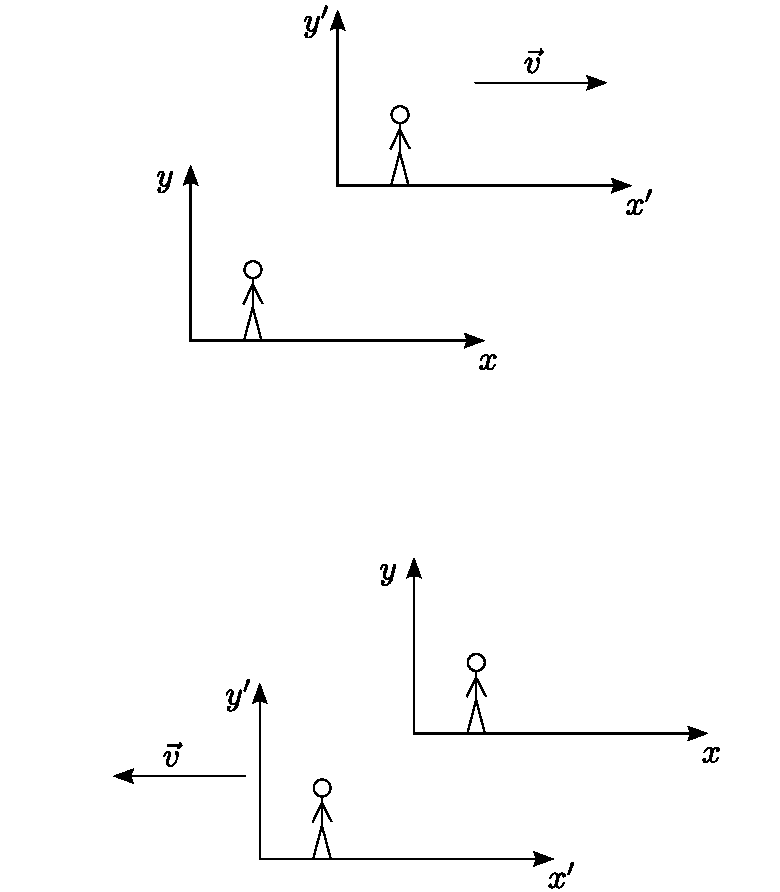
\includegraphics[width=\textwidth]{fig_7-7.pdf}
\captionof{figure}{Two reference frames: $(x,y)$ coordinates are used for the system defined to be at rest and $(x',y')$ coordinates are used for the system defined to be moving. In the upper figure, observer O is in the laboratory frame with observer P in the frame moving with velocity $v$. In the lower figure, the two systems have exchanged roles and $v\rightarrow-v$. All equations derived in the above system will be valid for the system below by exchanging $v\rightarrow-v$.\label{fig:deltat}}
%\end{center}
\end{Figure}

Going back to the example with the train: If the train moves at the speed $v=4c/5$ then we have $\Delta t=5/3\Delta t'\approx1.7\Delta t'$. When observer O on the ground watches the wristwatch of observer P, he notes that it takes $1.7$ hours on his own wristwatch before one hours has passed on the wristwatch of observer P. If observer P in the train is jumping up and down every second on his own wristwatch, it takes $1.7$ seconds for each jump as seen from the ground. For observers on the ground it looks like everything is in slow-motion inside the train.

How does it look for the observers in the train? Remember that velocity is relative. Being inside the train, we define ourselves as being at rest. From this frame of reference it is the ground which is moving at the speed $-v$. Everything has been exchanged: Since we now define the train to be at rest, the coordinate system $(x,t)$ is now for the train whereas the coordinate system $(x',t')$ is for the ground which is moving at velocity $-v$ (see figure \ref{fig:deltat}). Note the minus sign: The motion of the ground with respect to the train is in the opposite direction than the motion of the train with respect to the ground. 

We can now follow exactly the same calculations as above for two events happening at the position of observer O instead of observer P. For instance we watch two ticks on the clock of observer O. Then we find again formula (\ref{eq:deltat}) but with the meaning of $\Delta t$ and $\Delta t'$ interchanges. Assuming again a speed of $v=-4c/5$ (note again the minus sign), observer P sees that it takes $1.7$ hours on his wristwatch for one hour to pass on the wristwatch of observer O. It is the opposite result with respect to the above situation. While observers on the ground observe everything in the train in 'slow-motion', the observers on the train observe everything on the ground in 'slow-motion'. This is a consequence of the principle of relativity: There is no way to tell whether it is the train which is moving or the ground which is moving. We can define who is it rest and who is moving, the equations of motion that we obtain will then refer to one observer at rest and one observer in motion. When we change the definition, the roles of the observers in the equation will necessarily also change. Thus, if we define the ground to be at rest and the train to be moving and we deduce that observers on the ground will see the persons in the train in 'slow-motion', the opposite must also be true: If we define the train to be at rest and the ground to be moving, then the observers on the train will observe the observers on the ground in 'slow-motion'. Confused? Welcome to special relativity!

Consider two observers, both with their own wristwatch, one at rest in the laboratory frame (observer O) another moving with velocity $v$ with respect to the laboratory frame (observer P). Going back to equation (\ref{eq:deltat}) we now know that if $\Delta t'$ is the interval between two ticks on the wristwatch of observer P, then $\Delta t$ is the time interval between the same two ticks of observer P's watch measured on observer O's wristwatch. Using equation \ref{eq:deltat} we see that {the shortest time interval between two ticks is always the time measured directly in the rest frame of the wristwatch producing the ticks.} Any other observer moving with respect to observer P will measure a longer time interval for the ticks on observer P's wristwatch. This is of course also valid for observer O: The shortest time interval between two ticks on observer O's wristwatch is the time that observer O himself measures. The wristwatch time is called the {\it proper time} and is denoted $\tau$. It is the shortest interval between these two events that can be measured.

Note that the proper time between two events (two ticks on a wristwatch) also equals the spacetime interval between these events. This is easy to see: consider again the ticks on observer P's wristwatch. In the rest frame of observer P, the wristwatch is not moving and hence the spatial distance between the two events (ticks) is $\Delta x=0$. The time interval between these two events is just the proper time $\Delta \tau$. Consequently we have for the spacetime interval $\Delta s^2=(\Delta t')^2-(\Delta x')^2=\Delta \tau^2 - 0=\Delta \tau ^2$. 
\begin{formbox}
\textbf{Proper time}
\[
\Delta s^2 = \Delta \tau^2
\]
in the rest frame.
\end{formbox}

Now, let's return to another result, the length of the train $L$ as measured by observer O on the ground. Again, the result in equation \ref{eq:deltal} can be shown in a similar manner to be more general. The length $L_0$ can be the length of any object in the rest frame of this object. We see from equation \ref{eq:deltal} that {any observer which is not at rest with respect to the object will observe the length $L$ which is always smaller than the length $L_0$}. The length of an object measured in the rest frame of the object is called the {\it proper length} of the object. An observer in any other reference frame will measure a smaller length of the object. The proper length $L_0$ is the longest possible length of the object. This also means that an observer in the moving train will measure the shorter length $L$ for another identical train being at rest with respect to the ground (being measured to have length $L_0$ by observers on the ground).

\section{The Lorentz transformations}
\label{sect:lorentz}

Given the spacetime position $(x,t)$ for an event in the laboratory frame, what are the corresponding coordinates $(x',t')$ in a frame moving with velocity $v$ along the x-axis with respect to the laboratory frame? So far we have found expressions to convert time intervals and distances from one frame to the other, but not coordinates. The transformation of spacetime coordinates from one frame to the other is called the Lorentz transformation. In the exercises you will deduce the expressions for the Lorentz transformations. Here we state the results. We start by the equations converting coordinates $(x',y',z',t')$ in the frame moving along the x-axis to coordinates $(x,y,z,t)$ in the laboratory frame,
\begin{formbox}
\textbf{The Lorentz transformations}
\begin{align}
t&=v\gamma x'+\gamma t',\label{eq:florentz1}\\
x&=\gamma x'+v\gamma t',\label{eq:florentz2}\\
y&=y',\nonumber\\
z&=z'.\nonumber
\end{align}
\end{formbox}

To find the inverse transformation, we have seen that we can exchange the roles of the observer at rest and the observer in motion by exchanging the coordinates and let $v\rightarrow -v$ (see figure \ref{fig:deltat}),
\begin{formbox}
\textbf{The Lorentz transformations (cont.)}
\begin{align}
t'&=-v\gamma x+\gamma t,\label{eq:blorentz1}\\
x'&=\gamma x-v\gamma t,\label{eq:blorentz2}\\
y'&=y,\nonumber \\
z'&=z.\nonumber
\end{align}
\end{formbox}
Here 
\[
\gamma=\frac{1}{\sqrt{1-v^2}}.
\]

\section{List of expressions you should know by now}
\begin{tabular}{l c l}
Laboratory frame 	& $\rightarrow$ & page \pageref{pg:labframe}\\
Principle of relativity & $\rightarrow$ & page \pageref{pg:por}\\
Free float frame 	& $\rightarrow$ & page \pageref{pg:ff}\\
Space time diagram	& $\rightarrow$ & page \pageref{pg:spacetimediag}\\
Line element 		& $\rightarrow$ & page \pageref{pg:lineelement}\\
Lorentz geometry 	& $\rightarrow$ & page \pageref{pg:lorentz}\\
Spacetime interval 	& $\rightarrow$ & page \pageref{pg:spacetimeinterval}\\
Invariance 		& $\rightarrow$ & page \pageref{pg:invariant}\\
Proper time		& $\rightarrow$ & page \pageref{pg:propertime}\\
Proper length 		& $\rightarrow$ & page \pageref{pg:properlength}
\end{tabular}

\section{Introduction to the use of the 3D engine for relativity}

The MCAst 3D-application will be used for almost all the exercises in relativity. It is important that you now download the very last version of MCAst before embarking on the exercises. In these exercises, two and two students (and in some cases three students) are supposed to work together: Each student gets her/his frame of reference and is supposed to calculate what is going on in the other frame of reference. It is very important that you do not get tempted to download the videos of both frames, you will loose a significant part of the learning process by doing this: you need to agree with your partner who does which frame, then you download only your video. When you are done you will meet and look at each others videos and check your results.

Note that after starting MCAst, you can use the option 'settings' where can choose between using a GPU renderer, or switch off GPU using instead your computer's CPU. The graphics will be much better when using GPU, but it requires your computer to have a powerful graphics processor. {\bf Important:} the random generator is different between the GPU/CPU. This means that the landscape, events and the exercises in general will be different depending on whether you use CPU or GPU. It is therefore very important that you agree with you partner whether you will use GPU or CPU, both of you {\bf must} use the same.

In the upper left corner, there will be a clock showing the time in your frame of reference. There will also be a ruler on top to measure the position of events. The numbers which always appear next to the pointer shows the position measured on this ruler. The slider on the left can be used to adjust how fast the video plays, it is recommended that you run through the video fast the first time to see all events, then you run it much slower in order to measure time and position of events as exact as possible. Note that it will be very difficult to measure the exact time and position of the events. In these exercises you will notice the frustration of a real experimentalist: it is impossible to get exact numbers. We will not propagate errors in this course, but this is what would be done by a researcher when the numbers you measure are uncertain. Instead you will have to accept that there may be large errors in your answers, normally several percent. If you find that your calculated time and position of an event deviates by several percent from the answer shown in your partner's video, you know that this is to be expected and you can consider your calculation correct.

On the course web page, you will find a link to a list of xml-files which have the names of the exercises below as well as a specification of frame. Download the xml-file for your frame and put it in the data directory of MCAst. Then launch MCAst and you can load the xml and start the video.

Note: In almost all videos you can assume that the camera receives light from everything instantaneously (it is clearly written in the exercise when this assumption does not hold). This means that we have not taken into account the time it takes for light to travel from the planets/objects/events and to the camera. In this way, all the times and positions of the events are seen immediately as they happen. You therefore see events happening when and where they {\it actually} happen, but since light has a limited velocity a real observer would see some of the scenes quite differently. As an example, taking into account the effect of a non-zero light travel time a planet would not appear lenght contracted: it would still appear spherical but you would see the back side of the planets towards the edges.


\newpage


%\TileWallPaper{51.5pt}{11.5pt}{noisy_grid.png}
\section{Exercises}
\newcounter{problem}
\newcommand{\newproblem}[1]{\refstepcounter{problem}\label{#1}{\bf Exercise \refproblem{#1}}}

\newproblem{prob:lorentzyz}

We have seen the effect of Lorentz contraction, namely that a stick of proper length $L_0$ (measured in the rest frame of the stick) moving at a speed $v$ along the x-axis in the laboratory frame, is measured to have a shorter length $L=L_0/\gamma$ in the laboratory frame. But what happens to the size of the stick in $y$ and $z$ directions measured from the laboratory frame? Do we correspondingly measure the stick to become thinner? We will now investigate this:

\begin{Figure}
%\begin{center}
\centering
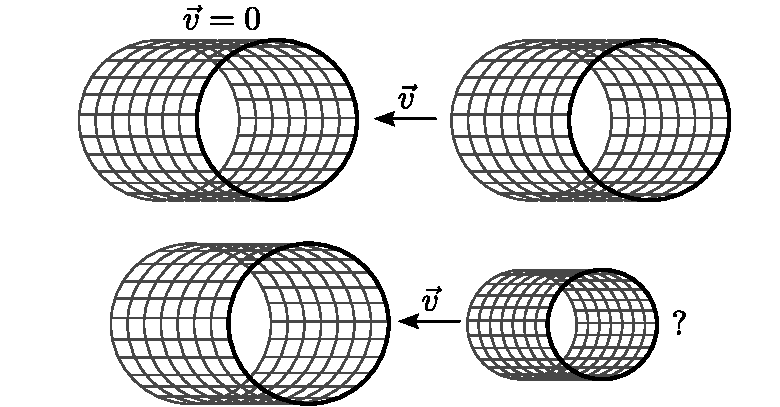
\includegraphics[width=\textwidth]{fig_7-8.pdf}
\captionof{figure}{Does a moving cylinder become thinner as well as contracted seen from the laboratory frame? In problem 1 we study this more closely.\label{fig:cylinder}}
%\end{center}
\end{Figure}

To check this possibility, imagine two identical cylinders A and B which are hollow such that if one cylinder becomes smaller (smaller radius) than the other, it might pass inside the larger cylinder (see figure \ref{fig:cylinder}). The axis of both cylinders are aligned with the x-axis at $y=z=0$. Thus, the axis of both cylinders are exactly along the x-axis. Cylinder A is at rest in the laboratory frame, cylinder B is moving with velocity v along the x-axis, approaching cylinder A. 

\begin{enumerate}
\item We know that the length of cylinder B as measured from the laboratory frame shrinks. Assume that the same effect takes place in the $y$ and $z$ directions such that the radius of cylinder B gets smaller measured in the laboratory frame. What happens when the two cylinders meet?
\item Now, look at exactly the same situation but from the point of view of an observer sitting on cylinder B. What happens when the two cylinders meet?
\item Can you give a good arguments to explain why $y=y'$ and $z=z'$ in the Lorentz transformations? (Note: this transformation is for movements along the x-axis. If there are movements along the y and z axes as well, the Lorentz transformation will look different and much more complicated. This is outside the scope of this course.) 
\end{enumerate}

%{\bf Problem 2 (10--20 min.)}

%A proton and an electron separated by a distance $L_0$ are at rest in a train. 
%\begin{enumerate}
%\item What is the electric field $E'$ from the proton at the location of the electron? (as measured in the rest frame of the train)
%\item The train moves with velocity $v$ with respect to the laboratory frame. Show that the electric field $E$ as measured in the laboratory frame can be written as $E=E'/(1-v^2)$.
%\item Based on this result, can you now use the principle of relativity to find  general qualitative arguments showing that the electric feld must be a relative quantity depending on the frame of reference in which it is measured?
%\end{enumerate}

\vspace{0.5cm}


\newproblem{prob:cosmicray}

You need to have read sections \ref{sect:simul} - \ref{sect:oandp} to be able to do this exercise. We will look at a spaceship trying to land on a planet, but failing and crashing. One unlucky observer sits in the space ship, another one is on the ground, being hit by the crashing space ship. Go to MCAst and load the xml corresponding to this exercise. There are two frames, one xml for each, you and your partner should agree on who does which frame. 

In the upper left corner the time in your frame of reference is shown.  The best way to read off the exact time of events is to stop the video and then slide the slider manually, stopping just before the events are occuring and then play the video in slow motion (which is standard but can be changed with the speed slider) in order to stop exactly when the events occur and thereby read off the exact time.

Your main task is to calculate how long it takes from the space ship enters the planet's atmosphere untill it crashes on the ground, {\bf measured on the clock in the other frame of reference}. In the upper left corner you are given a message when the space ship enters the atmosphere, as well as when the space ship has crashed. These messages show exactly when the events are happening.

Note that uncertainties in reading off values may give errors up to a few percent on the numbers you obtain, errors of this order are to be expected and are accepted.

\begin{enumerate}
\item How long time does it take {\bf in your frame of reference} from the moment the space ship enters the atmosphere until it crashes?
\item In your frame of reference, how large distance does the space ship travel from the beginning of the atmosphere to the ground? When the message about the space ship entering the atmosphere appears, also the distance from the beginning of the atmosphere to the ground is given.
\item What is the velocity of the space ship?
\item Calculate the space time interval between these two events in your frame of reference, give the answers in ms ($10^{-3}$s).
\item Write an expression for the same space time interval in the other frame of reference and use invariance of the space-time interval to calculate the time it takes from the space ship enters the atmosphere until it crashes in {\bf the other frame of reference}.
\item  When high energy cosmic ray protons collide with atoms in the upper atmosphere, so-called muon particles are produced. These muon particles have a mean life time of about $2 {\rm \ \mu s}$ ($2\times10^{-6} {\rm \ s}$) after which they decay into other types of particles. They are typically produced about 15~km above the surface of the Earth. We will now study a cosmic ray muon approaching the surface with the velocity of $0.999c$. How long time does it take for a muon to arrive at the surface of the Earth as measured from the Earth frame?
% 50 mus
\item Ignore relativistic effects: Do you expect many muons to survive to the surface of the Earth before decaying? (compare with the mean life time)
\item Now use invariance of the space-time element (exactly as you did for the space ship above), to find the time it takes to reach the surface of the Earth in the rest frame of the muon. Does it change your conclusion on the previous question?
\end{enumerate}

\vspace{0.5cm}


\newproblem{prob:timedilat}

Go to MCAst and load the xml corresponding to this exercise. There are two frames and one xml for each, you and your partner should agree on who does which frame.

A space ship is travelling in the atmosphere of a planet and there are 3 lightenings occuring. One frame of reference is the frame of the space ship where lightenings will take place at positions $(x',t')$. The other frame is the frame of the planet with lightenings taking place at $(x,t)$. The relative velocity between the planet and the space ship is given in the upper left corner. Use the ruler at the top, or just look at the (x,y) position shown with the cursor to find the position of events. In some cases it may be difficult to read the numbers close to the event, in this case just move the cursor straight upwards where the background is black. The best way to read off the exact times and positions of events is to stop the video and then slide the slider manually, stopping just before the events are occuring and then play the video in slow motion (which is standard but can be changed with the speed slider) in order to stop exactly when the events occur. Note that a white ball is put in the middle of the lightening in order to make it easier to read off the exact positions.

 In this exercise we will focus at the yellow and the blue lightenings which both strike the space ship. The purpose of this exercise is to measure the time difference between the two strikes in your frame and use invariance of the space-time interval to calculate the time interval in the other frame. In the following, it is important that you try to measure the exact time when the events happen. The space ship is always in position $x'=0$ in the space ship frame, and both lightenings happen exactly at the position of the space ship.

Note that uncertainties in reading off values may give errors up to a few percent on the numbers you obtain, errors of this order are to be expected and are accepted.


\begin{enumerate}
\item First we will make a test of MCAst on your computer: stop the slider exactly when the pink lightening strikes (we will use the pink lightening just for this test). Try to move the time slider so that you stop exactly at the moment when the lightening first appears. There is a number appearing with the event telling the position of the event. Move the cursor in the middle of the pink lightening and see if the number which appears next to the cursor (which is the exact x-position from the ruler on top) is very similar to the number appearing in the text for the event. If the discrepancy is large, you should immediately contact your teacher/group teacher to check if something is wrong with the installation on your computer (this happens on some systems)
\item {\bf For both frames:} 
\begin{enumerate}
\item In your frame, at what time $t_1$ and $t_2$ do the lightenings strike? 
\item In your frame, at what positions $x_1$ and $x_2$ do the two lightenings (yellow and blue) strike? 
\item What is the time interval between the two lightenings?
\end{enumerate}
\item {\bf For the frame of the space ship:}
\begin{enumerate}
\item Can you express the position of the two lightenings, $x_1$ and $x_2$ (as measured in the frame of the planet) in terms of the relative velocity $v$ and the (for you) unknown times $t_1$ and $t_2$ which are the times when the two lightenings strike measured on the clock in the planet frame? {\bf Hint:} At $t=0$ the origin of both systems are aligned: look at the landscape just below the space ship at this moment. This point in the landscape corresponds to $x=0$ in the frame of the planet. At any later time $t$, what is the position of the space ship $x$ at that moment measured in the planet frame? Since both events take place at the position of the space ship, you can use this information to find the position of the lightenings.
\item Use the invariance of the space-time interval to find the time interval $\Delta t_\mathrm{12}$ between the two lightenings as measured in the planet frame.
\item Repeat the previous question, but now write $\Delta t$ for the time interval in the planet frame and $\Delta t'$ for the time interval in your frame (do not insert numbers). Do you find the expression for time dilatation?
\end{enumerate}
\item {\bf For the frame of the planet:}
\begin{enumerate}
\item What are the positions $x_1'$ and $x_2'$ for the two lightenings in the frame of the space ship?
\item Use the invariance of the space-time interval to find the time interval $\Delta t_\mathrm{12}'$ between the two lightenings as measured in the frame of the space ship.
\item Repeat the previous question, but now write $\Delta t$ for the time interval i the planet frame and $\Delta t'$ for the time interval in the space ship frame (do not insert numbers). Do you find the expression for time dilatation? {\bf Hint:} you will need to find an expression for the positions $x_1$ and $x_2$ of the lightenings in your frame, as a function of velocity $v$ and time of events $t_1$ and $t_2$. Use your numbers to check if your expressions are correct.
\end{enumerate}
\item Now meet your partner and look at your videos together. Your partner has the answers to your calculations. While you watch both videos simultaneously, look at the landscape to see the position of the space ship at both events. Although it might be difficult to see, they should both occur above the same positions in the landscape. Look at the distance between these two positions. In which frame is the distance between the two lightenings (and thereby between the two points in the landscape) larger?
\end{enumerate}

\vspace{0.5cm}



\newproblem{prob:simultaneity}

In this problem we will study two spaceships moving at the same speed with respect to the ground. In the frame of the space ships, both space ships simultaneously shoot a laser beam towards the other (event A and B, left space ship shooting is event A). These two events are not simultaneous in the ground frame. When the laser beams hit, the ships explode (event C and D, leftmost explosion is event C), creating two more events. In this exercise, we will study all these 4 events from the two different frames of reference.

Event A, the emission of the laser beam from the leftmost space ship, takes place at $x=x'=0$ and $t=t'=0$ in both frames.

In this exercise you are working alone. Go to MCAst and load the xml
corresponding to the space ship frame which is frame 1 for this
exercise. Do {\bf not} look at the video for the planet frame (frame 2) at this moment.


\begin{enumerate}

\item We see that the emission of laser beams are simultanous in the
space ship frame. The same goes for the two explosions. Imagine that
you do not know about the theory of relativity, but you know that the
velocity of light is the same for all observers. Imagine an observer
which is situated in the middle bertween two space ships and which is
at rest in the space ship frame. We call this oberver M(iddle) which
is also visible in the video({\bf Johan og Jon vi m\aa\ legge inn
denne i videoen}. Observer M will see the two sets of events as simultaneous, i.e. the laser beams will cross exactly at her position. Why? Check in MCast that this is really the case.

\item Now we will try to figure out what happens in the planet frame
without having looked at the video:  Assume we do not know about
 length contrations and time dilations. We therefore believe that the
 distance between the two space ships is still the same in the planet
 frame. Using that
\begin{itemize}
\item we know observer M sees the two light beams crossing
 just at her position (why must this be the case in both frames?),
\item  the fact that observer M is in the middle between the space ships,
\item  that the laser beams were emitted simultaneously in the space
ship frame, 
\end{itemize}
we can conclude that in the planet frame, the laser beams where not
emitted simultaneously, but at two different times. Why?
Try to think how the space ship and observer M are moving while the
laser beams are emitted.

\item Again imagine the situation as seen from the planet frame: In
order for the laser beams to cross exactly at the position of observer
M, which of the laser beams must have been emitted first in the planet
frame? Why? Again imagine the movements of the space ships and the
laser beams in the planet frame.

\item Turning to the explosions, could these still be simultaneous?
In the space ship frame they happen at the same time at the same
distrance from observer M. Therefore the light from the explosions
will reach observer M at the same time and observer M will observe
both explosions simultaneously. Can the explosions be simultaneous in
the planet frame? Repeat the above line of thought.

\item Now repeat the above reasoning and find out which of the
explosions must have happened first. It is easy to conclude too fast
here, think twice before answering.

\item Now order events A, B, C and D in chronological order in the
planet frame. Write a short summary of why this has to be the order of
the events using the reasoning we learned above. Imagine how this will
look. Then {\bf only after you
have really tried to imagine how this looks}, look at the video for
the planet frame.

\item We will in the following use invariance of the space-time interval to
calculate the exat time and position of the events in the planet
frame. Make a list of the times $t'$ and positions $x'$ of all four
events in the space ship frame, all expressed in km. Also calculate the distance $L'$
between the space ships in the space ship frame. We will call the
unknown distance between the space ships in the planet frame $L$.

\item Write the times and positions of these same 4 events in the
planet frame, expressed in terms of the unknown planet frame
quantities $t_B$, $t_C$, $t_D$ and $L$. Use the video for the
planet frame (not using numbers just qualitatively looking at what is happening) as assistance to find
expressions for $x_B$, $x_C$ and $x_D$.{\bf Jon og Johan: vi vil ikke
at tidspunkt og posisjon til eventene skal vises p\aa\  skjermen i frame 2
her}

\item Make a function for the position of the laser beam emitted in event A as a function of time. Use this function together with a function for the position of the rightmost space ship to find an expression for the time $t_D$ of event D expressed in terms of the unknown $L$ as well as the velocity. Find also an expression for $x_D$.
\item Use invariance of the space-time interval $\Delta s_{AC}$ to find a value for the time $t_C$ of event C expressed for the moment in km. Use this to find $x_C$, also in km.
\item  Make a function for the position of the laser beam emitted in event B as a function of time. Use this function together with a function for the position of the leftmost space ship to find an expression for the time $t_B$ of event B expressed in terms of the unknown $L$. Find also an expression for $x_B$.
\item Use invariance of the space-time interval $\Delta s_{BD}$ to
find the value of $L$. This calculation might be long and ugly if you
don't do it right: Wait by inserting the expressions you have for
$t_B$ and $t_C$ until you have simplified the expression as much as
you can.
\end{enumerate}

In the second part of this exercise, we will now again imagine that we
do not know about length contraction and time dilation. Our goal now
is to try to imagine being Einstein when he just discovered
relativity. Using only the fact that the speed of light is the same in
both frames, we will try to arrive at the expression for time dilation
using the situation with the space ships and pure reasoning. Be
prepared that we might not quite arrive though.

In the following we will not use numbers, only symbols for times,
positions and distances in the planet frame.

\begin{enumerate}

\item Write the planet frame positions of the two space ships,
observer M as well as the two laser beams, all as functions of (1) time $t$ in the planet frame, (2) the time $t_B$ when the laser was emitted from the rightmost ship, (3) the distance $L$ between the space ships and (4) the velocity $v$ of the space ships with respect to the ground (remember that the leftmost beam was emitted at time $t=0$). In particular, show that the position of the laser beam moving to the left is given by $x_\mathrm{beam2}=L+vt_B-(t-t_B)$.
\item Use these functions to show that the time $t_X$ when the two
laser beams cross at the position of observer M (in the middle between the two space ships) can be written as $t_X=\frac{L/2}{1-v}$.
\item Use the fact that position of the beam moving to the left at
time $t=t_X$ equals the position of observer M at the same time $t_X$ to show that $t_B=t_X-\frac{L/2}{1+v}$.
\item Use the fact that the explosion of the left space ship (event C) happens when the position of the beam moving to the left equals the position of the left space ship to show that $t_C=t_X+\frac{L/2}{1+v}$.
\item Now imagine that in the explosions, light beams from the
explosion are sent towards observer M. Again, the two explosions were
simultaneous in the space ship frame such that the observer sees the
two explosions simultaneously (the light beams from the explosion
cross at the position of observer M). Show that the position of the light from the explosion of the left space ship can be written as $x_\mathrm{light}=vt_C+(t-t_C)$.
\item At time $t_{X2}$ (planet frame time), the light beams from the
two explosions cross at the place of observer M. Use the position of the light which you found in the previous question to show that $t_{X2}=t_X+\frac{L}{1-v^2}$.
\item What is the time interval $\Delta t=t_{X2}-t_X$ in the planet frame? This is the time interval between when observer M sees the two laser beams crossing and when the observer sees the two explosions.
\item Show that the corresponding time interval in the space ship
frame (the time interval that observer M actually measures on her clock between these events) is given by $\Delta t'=t'_{X2}-t'_{X}=L$.
\item What is the ratio between $\Delta t'$ in the space ship frame and $\Delta t$ in the planet frame? Does it look similar to the expression for time dilation in special relativity? Why is it different? Having our (wrong) assumptions in mind, and knowing the real formula for time dilation, could you actually have guessed this result?
\end{enumerate}




\vspace{0.5cm}


\newproblem{prob:mirrorclock}

You need to have read sections \ref{sect:simul} - \ref{sect:oandp} to be able to do this exercise. We will play cosmic ping-pong with laser beams: two space ships are at a fixed distance $L'$ apart (in the reference frame of the space ships). Both space ships travel with the same velocity with respect to the planet below. At $t=t'=0$ the space ship situated at $x=x'=0$ emits a laser beam towards the other space ship. At this moment the space ship emitting the beam is passing a space station (white disk) behind. The space station is in the same frame of reference as the planet and positioned at $x=0$ in that system. Both space ships have mirrors in front so that the laser beam will now be reflected backwards and forwards between the two space ships.

We will call the emission of the beam event A, the first reflection on the other space ship is event B and the second reflection at the point where the beam was emitted is event D. There is also an event C: an explosion which happens at the space station at the same moment as event B happens in the frame of reference of the space ships. We will use coordinates $(x,t)$ for the planet frame and $(x',t')$ for the space ship frame. The relative velocity between the two systems is given in the upper left corner.

In this exercise you are working alone. Go to MCAst and load the xml
corresponding to the space ship frame which is frame 1 for this
exercise. Do {\bf not} look at the video for the planet frame (frame 2) at this moment.

\begin{enumerate}

\item In the first questions you are only supposed to do reasoning, no calculations, to arrive at your answers. In particular we will compare the time it takes for the laser beam to go from left to right, compared to the time it takes to go from right to left, i.e. compare $\Delta t_\mathrm{AB}$ to $\Delta t_\mathrm{BD}$. Suppose you instantly hear a bell sound each time the laser beam hits a mirror: in the frame of the space ships you will clearly hear the bell sound with a constant frequency (why?). Now imagine how this looks in the planet frame, remembering that the speed of light is the same in all frames of reference and that the space ships are moving at a speed close to the speed of light. Will an observer in the planet frame hear the bell sounds with a constant frequency? If not, how does it sound? Which of $\Delta t_\mathrm{AB}$ and $\Delta t_\mathrm{BD}$ are longer?

\item Now we will look at a similar situation in a non-relativistic setting: suppose the laser beam is a ping pong ball moving at $80$km/h with respect to the space ships and the space ships are moving at $50$km/h with respect to the planet. Again, do not make any calculations, only reasoning: what will you hear in the planet frame? Is the answer similar or different from the case with the laser beam? Give reasons for your answer.{\bf Jon og Johan: trenger vi å lage en video for å illustrere dette ogs\aa ?}

\item Looking again at the same situation as the previous question, but this time the ball moves with  $50$km/h with respect to the space ships. Again with no calculations, can you explain how this will look from the planet frame?

\item Suppose we increase the speed of the ball and the space ships such that both are getting closer and closer to the speed of light. Will the observer in the planet frame hear the bell sounds with constant frequency all the time untill the ball is replaced by a laser beam? Or will the frequency become gradually less constant as the speed increases? At the moment you can speculate, then you should revisit this question after reading part 2B on velocity transformations.

\item Before starting the calculations there is one more question you are supposed to solve using only reasoning: Go back to the situation shown in the video with a laser beam going back and forth between the space ships and with an explosion at the space station: Event C is simultaneous with event B in the frame of the space ships. We know that events which are simultaneous in one frame cannot be so in another frame. In the planet frame, will event B happen before event C or vice versa? {\bf Hint:} Try to insert a space ship frame observer which is just in the middle between event B and C when these two events happen. You may suppose that this observer is not very close to any of the space ships as seen from the planet frame when any of these events happen  (if we do not suppose this, could the conclusions change? Why?).

\item Look at the video for the planet frame and check your answers.{\bf Jon og Johan: vi vil ikke at tidspunkt og posisjon til eventene skal vises p\aa\  skjermen i frame 2 her}

\item Now we will calculate the exact times between the events and find out at what time the bell sounds will be heard in the planet frame. Start by using the video for the space ship frame to write the time $t'$ and position $x'$ of all events in the space ship frame. Use these to find the distance $L$ between the space ships as well as the time intervals between the first reflections, $\Delta t'_\mathrm{AB}$ and $\Delta t'_\mathrm{BD}$ in the space ship frame.

\item Now our task will be to find $\Delta t_\mathrm{AB}$ and $\Delta t_\mathrm{BD}$ in the planet frame: We will do this step by step in the following questions. Start by writing down the positions and times of events in the planet frame which you know by simple reasoning. Some positions may be expressed through the velocity and the unknown time of an event in order to reduce the number of unknowns. The only unknowns should be $x_B$, $t_B$, $t_D$ and $t_C$, other unkown positions and events should be written in terms of these. {\bf In this exercise you should express all numbers in units of time, it is convenient to convert all distances to ms.}
\item Write the spacetime intervals $\Delta s_{AB}$ and $\Delta s_{AB}'$ between events A and B in the two frames. Show that invariance of the interval gives $x_B=t_B$ in the planet frame. Could you have guessed this using physical arguments without any calculations?
\item  Write the spacetime intervals $\Delta s_{AC}$ and $\Delta s_{AC}'$ between events A and C in the two frames. Show that invariance of the interval gives a number for $t_C$ in the planet frame. 
\item Write the spacetime intervals $\Delta s_{BC}$ and $\Delta s_{BC}'$ between events B and C in the two frames. Show that invariance of the interval gives $t_B$ in the planet frame.
\item Use invariance of the spacetime interval for appropriate events to find at what time $t_D$ event D happened in the planet frame. 
\item In the planet frame, how long time did it take from the light was emitted to the first reflection? 
\item How long time did it take from the first reflection to the second reflection?
\item Which event happened first in the planet frame, event B or C? Is it consistent with you reasoning above?
\end{enumerate}




\newproblem{prob:lorentztrafo}

You need to have read sections \ref{sect:simul} - \ref{sect:oandp} to be able to do this exercise. In this exercise we will deduce the Lorentz transformations using only invariance of the space-time interval. Load the xml corresponding to this exercise which are very similar to the ones used in exercise \refproblem{prob:timedilat}. You should read the introduction to that exercise again to repeat the basic information about these videos.

In the space ship frame, the space ship is always at position $x'=0$. In the planet frame, the space ship starts at $x=0$ and moves along the positive x-axis. In the space ship frame: note at which point in the landscape above which the space ship starts. Remember that this is the origin $x=0$ in the planet frame. When the space ship moves, this point in the landscale moves backwards, but remember that from an observer on the ground, the space ship moves along the positive x-axis.

Our main task here is to deduce the time and position of the pink lightening in the other frame using only information obtained from observations in our own frame as well as the invariance of the space-time interval. In order to archieve this, we will make use of 3 more events, 3 lightenings, green, yellow and blue, two of which hit our space ship. We have constructed these additional events such that in the planet frame, one lightening hits the space craft simultaneously with the occurence of the pink lightening. In the space ship frame, one lightening occurs simultaneously with the pink lightening at the position of the origin of the x-axis in the planet frame (remember this point in the landscape, although the new angle will make it appear in a slightly different position). The green lightening occurs at $t=t'=0$ at position $x=x'=0$ in both frames.

 We call the green lightening ``event 0'', the pink lightening ``event 1''. The blue lightening which occurs simultaneously with event 1 in the planet frame is called ``event 2a'' and the yellow lightening which occurs simultaneously with event 1 in the space ship frame is called ``event 2b''. The positions in the planet frame are denoted $(x,t)$ and in the space ship frame $(x',t')$. Both students will only need to use 3 events in this exercise: both students need the green and the pink lightening (event 0 and 1) as well as the lightening occuring simultaneously with the pink lightening in their frame (event 2).

We repeat again that the main final goal for the following questions is to deduce the time and position of the pink lightening in the other frame

\begin{enumerate}
\item Use the video to measure and write the time and position for all 3 events in the coordinates of your frame of reference as well as in the other frame of reference. Your task is to find the time and position of event 1 (the pink lightening) in the other frame of reference. Note that also the time of event 2 in the other frame is unknown. The position of event 2 in the other frame is known.
\item Use invariance of the space-time interval $\Delta s_{02}$ and $\Delta s_{02}'$ to find the time of event 2 in the other frame.
\item Use invariance of the space-time interval $\Delta s_{01}$ and $\Delta s_{01}'$ to find an expression for the position $x_1$ of event 1 in the other frame, expressed in terms of the unknown time $t_1$ of event 1 in the other frame.
\item Use invariance of the space-time interval $\Delta s_{12}$ and $\Delta s_{12}'$ and insert the expression from the previous question to eliminate the position $x_1$ in the other frame. Also the second order terms of the time $t_1$ in the other frame should vanish. You should now easily obtain a number for the time $t_1$ for event 1 measured in the other frame.{\bf Important:} You should not get a second order equation here. If you do, you have got one of the events wrong: look carefully at the videos again and read carefully the information given at the beginning of this exercise.
\item Now use this time to obtain a number for the position $x_1$ of event 1 on the other frame.
\item You and your partner student should now compare numbers: He/she should have found the position and time of the pink lightening in your frame and you should have found the position and time of the pink lightening in his/her frame. Look at both videos together and observe in particular event 2 which is different for both of you.
\item Now here is the main point of this exercises: we will now deduce the Lorentz transformations using event 1: The Lorentz transformations are two equations relating $x,t$ for an event in one frame with $x',t'$ for the same event in another frame. Here we will use event 1 and thereby deduce the relation between $x_1,t_1$ and $x_1',t_1'$ where the relation also contains the velocity $v$ between the frames. Go back and repeat the previous questions, but now instead of inserting numbers, use letters:
replace numbers with the following letters, $x_1$, $t_1$, $x_1'$, $t_1'$ as well as the time of event 2 in the other frame. Some of the times/positions are 0, these should not be replaced by letters. These 5 letters will be your unknown and you should not need to introduce more unknowns. {\bf Hint:} You will need to write the position of event 2 in your frame in terms of the velocity $v$ of the other frame as well as the time of event 2 in your frame. Look back at exercise \refproblem{prob:timedilat} and see how a similar task was done there. Now write the events in terms of these letters and repeat the above calculations using the same space-time intervals.
\item The student in the space ship frame should have obtained the expression for the forward Lorenz transform (equations \ref{eq:florentz1} and \ref{eq:florentz2}), and the student in the planet frame should have obtained the expression for the backward Lorenz transform  (equations \ref{eq:blorentz1} and \ref{eq:blorentz2}).
\end{enumerate}


\vspace{0.5cm}

\newproblem{prob:lorentztrafo2}

You need to read section \ref{sect:lorentz} before doing this exercise. We will now return to the cosmic ping-pong in exercise \refproblem{prob:mirrorclock} and solve this using the Lorentz transformations instead of the spacetime interval. Your task is again to calculate the time intervals $\Delta t_{AB}$ and $\Delta t_{BD}$ in the other frame of reference. Using the Lorentz transformations we will only need events A, B and D.

\begin{enumerate}
\item Again, write up the coordinates $(x,t)$ and $(x',t')$ for these three events, some as numbers, some expressed through other coordinates. The following are unknown: $x_B$, $t_B$ and $t_D$ in the other frame of reference.
\item Use the Lorentz transformations to find $t_B$ and $t_D$. You do not need to find $x_B$.
\item Now find  $\Delta t_{AB}$ and $\Delta t_{BD}$ in the other frame of reference.
\end{enumerate}

\newproblem{prob:twinparadox}


We will finish this lecture by studying the twin paradox in detail. This long and detailed exercise is very important to gain some basic understanding for the underlying physics of many of the so-called paradoxes in the theory of relativity. You need to have read sections \ref{sect:simul} - \ref{sect:lorentz} to be able to do this exercise.
There are three xml files for this exercise and you need to be three students doing this exercise together: you need to meet already from the beginning and do everything together. {\bf Please note that you will really loose many important points if you do this exercise alone, in particular it is important to be able to see the different videos at the same time without having to switch continously between xml files.}

You are an astronaut traveling from planet P1 to planet P2 in another star system 200 light years from planet P1. You start at $x=x'=0$ and $t=t'=0$ where $(x,t)$ are planet frame coordinates and $(x',t')$ are spaceship coordinates. You travel in your spaceship at a velocity of $v=0.99$. We assume that the planets do not move with respect to each other and that they therefore are in the same frame of reference. Frame one shows everything from the planet frame, focusing all the time on planet P1. Frame two is the frame of reference of the space ship. The third frame is the frame of reference of a second space ship travelling from planet P3, passing planet P2 and arriving at planet P1. Planet P3 is a planet in yet another star system being 200 light years away from planet P2 and 400 light years away from planet P1. Planet P3 is also in the same frame of reference as planet P1 and P2. The velocity of the second space ship is $v=-0.99$ in the opposite direction of the first.

We will start focusing only on planet P1 and P2 and the first space ship travelling between these. To solve these first questions, you are not supposed to use MCAst:


\begin{enumerate}
\item Event A is you departing from planet P1. Event B is you arriving on planet P2. In the planet frame it took $200/0.99\approx202$ years to arrive at planet P2. We know that for you it took a factor $\gamma=1/\sqrt{1-v^2}$ less ($\Delta t=\gamma\Delta t'$, $\Delta t$ is measured in the planet frame, $\Delta t'$ is measured in spaceship frame). How long time did it take for you (on your wristwatch) to arrive on planet P2?
\item After arriving on planet P2, you make the necessary scientific measurements (which takes very little time and can therefore be ignored) and start the return flight. You fly with exactly the same speed $v=0.99$ towards planet P1. Event C is when you arrive back on planet P1. Use the same arguments (or symmetry arguments) to find the time $\Delta t$ and $\Delta t'$ it took from planet P2 and back to planet P1 in the two frames of reference.
\item If you have done your calculations correct, here is a summary of the situation: In the planet frame, it took you $404$ years to go to planet P2 and return. On your wristwatch it took you 57 years to go to planet P2 and back. So while hundreds of generations have passed on planet P1, you return 57 years older.
\item We will now make the same calculations again, but just switch the frames: The laboratory frame $(x,t)$ is now the frame of the spaceship and the moving frame $(x',t')$ is the planet frame. Because of the principle of relativity we are allowed to switch the roles and we should arrive at exactly the same result using the same laws of physics. From this point of view, this is what is happening: You sit in you spaceship which is now the laboratory frame defined to be at rest and at $x=x'=0$ at $t=t'=0$ (event A), planet P1 starts moving away from you with velocity $v=0.99$ and planet P2 starts approaching you with the same velocity. After a time $\Delta t$ planet P2 arrives at your position (event B). We know from previous calculations that the trip took $28.5$ years in your frame of reference which is now the laboratory frame. Using again that $\Delta t=\gamma \Delta t'$ (and make sure not to confuse $\Delta t$ and $\Delta t'$) show that the clocks on planet P1 at the moment when planet P2 arrives at your position show 4 years. Only $4$ years had passed on planet P1 during the $28.5$ years (on your watch) trip to planet P2.
\item  Now, this might look like a paradox, but we will show further down that it is not. No matter how strange this might sound, it is consistent. The paradox is still to come. After making your investigations of planet P2, planet P2 departs and planet P1 approaches you again at the speed of $v=0.99$. Making the same calculations again you will find that it takes planet P1 $28.5$ years to return to you. Let's again check carefully how long it takes on the planet P1 clocks for planet P1 to return to your position: At the moment you  have finished your investigations, the planet P1 clocks show $t'=4$ years and your clock shows $t=28.5$ years. It takes planet P1 again $\Delta t=28.5$ years to arrive at your position. We have as always that $\Delta t=\gamma \Delta t'$. How long did it take for planet P1 to return to your position measured on planet P1 clocks?
\item If you made the last calculation correct, this is now the situation: It took you 57 years from planet P1 departed to planet P1 returned. However, on planet P1 clocks it took $8$ years. So while you are 57 years older, only $8$ years have passed on planet P1. Above we found that $404$ years had passed on planet P1. Now, this is a paradox!
\item Clearly we made an error somewhere in the calculations. Or maybe we simply forgot some basic principles from special relativity? It appears at first sight that the two roles are equal, that we can choose whether we consider the planet frame as the laboratory frame or the spaceship frame as the laboratory frame. But are the two roles really identical? What is the difference between the two observers, the planet P1 observer and the spaceship observer?
\item Don't read on until you have found an answer to the previous question. Here comes the solution: The difference is that whereas the planet P1 observer always stays in the same frame of reference, the spaceship observer changes frames of reference: The spaceship needs to accelerate at planet P2 in order to change direction and return to planet P1. Planet P1 does not undergo such an acceleration. The expression $\Delta t=\gamma \Delta t'$ was derived for constant velocity (look back at its derivation). It is not valid when the velocity is changing. In order to solve this problem properly one needs to either use general relativity which deals with accelerations or we can view the acceleration as an infinite number of different free float frames, frames with constant velocity, and apply special relativity to each of these frames. We will not do the exact calculation here, but we will do some considerations giving you some more understanding of what is happening. We will now consider three frames of reference. The planet P1 frame $(x,t)$, the outgoing spaceship frame $(x',t')$ and the returning spaceship frame $(x'',t'')$. Instead of spaceships we will look at it as space ship elevators going between planet P1 and planet P2. There are an infinite number of space ships going in a line with fixed distance between the two planets. At $x=x'=0$ and $t=t'=0$ you start in one of these space ships at planet P1 going in the direction of planet P2. There are other observers in the other space ships before you and after you. The situation is depicted in figure \ref{fig:elevator}, in this illustration as an elevator. In the following questions you may use the Lorentz transformations to transform between the coordinate systems when necessary. We write the distance between planet P1 and P2 in the planet frame as $L_0$. Event A happens at $x_A=x_A'=0$ and $t_A=t_A'=0$. Event B is again the moment when you arrive at planet P2. At what time $t_B$ in the planet frame do you arrive at planet P2? (express the answer in terms of $L_0$ and $v$)
\begin{Figure}%[tbp]
%\begin{center}
\centering
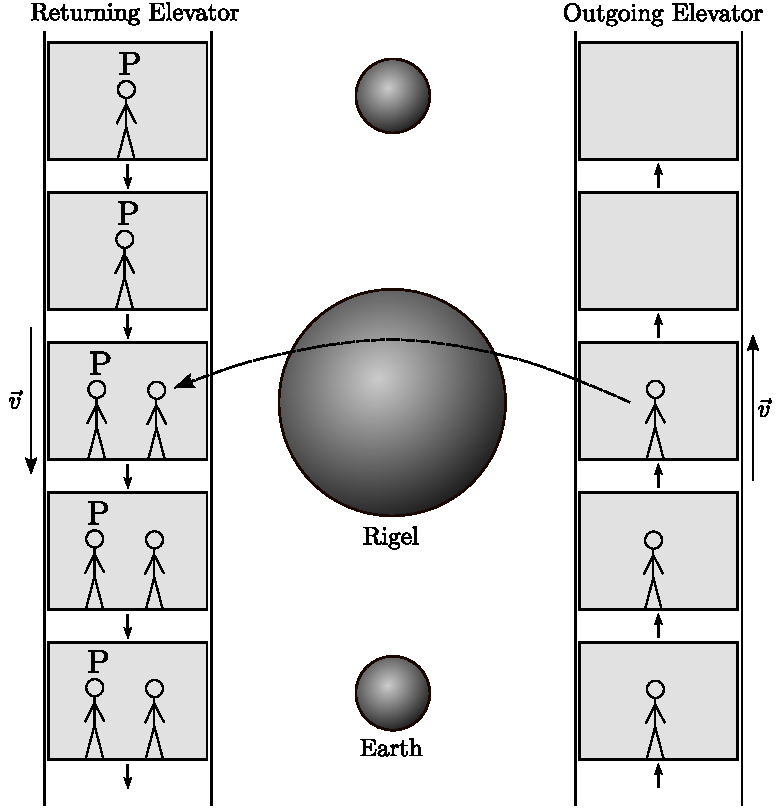
\includegraphics[width=\textwidth]{fig_9-5.pdf}
\captionof{figure}{The elevator between planet P1 and planet P2.\label{fig:elevator}}
%\end{center}
\end{Figure}
\item Now is the time to look at the videos: The outgoing spaceship is yellow. When arriving on planet P2, the astronaut is launching himself from the yellow to a red spaceship in the incoming space ship elevator using a spherical space capsule. Then the astronaut returns to planet P1 in the red space ship. In these videos, you are {\bf not} supposed to use the usual clock in the upper left corner. Instead there is another clock just below which counts years. This clock shows the time in your frame of reference. Note that the video will, at some points, make a fast forward run.
\item Use the Lorentz transformations to find $t_B'$, the time on your wristwatch when you arrive on planet P2. Insert numbers and check that you still find that the trip takes $28.5$ years for you. Compare with the space ship clocks in the video of the space ship frame.
\item We now define event B'. At the same time as you arrive at planet P2  (in your frame of reference which is now the frame of the outgoing elevator), another observer in another space ship in your elevator (thus another observer in your frame of reference using clocks synchronized with yours) passes planet P1 at position $x_{B'}=0$. Event B' is the event that he looks out and checks what time it is on planet P1. When doing this, he turns on a blue light on his space ship, you will see this in the video of the frame of planet P1. So event B' takes place at the position of planet P1, but at the same time as you arrive at planet P2 (same time in the outgoing reference frame). Show that the time $t_{B'}$ which he reads off the planet P1 clocks can be written as $t_{B'}=L_0/v-vL_0$. Insert numbers. {\bf Hint:} You first need to find the position $x_{B'}'$ of event B' in the outgoing elevator frame.
\item Insert numbers in your previous result and compare to the time you measure in the video (which time does the astronaut read off the Earth clocks when turning on the blue light?). Explain the result which we found earlier when using the spaceship as the laboratory frame: Namely that when planet P2 arrived at the spaceship, we calculated that on the planet P1 clocks only $4$ years had passed. Why is this not a surprise? Those who were surprised earlier, do you now understand which error you made when you got surprised? Which basic principle of relativity had you forgotten?
\item We learned in the previous question that even if the P1 clocks were observed at the same moment as the spaceship/elevator arrived at planet P2 (in the outgoing frame), these two events (the observation of the P1 clocks and the arrival at planet P2) were \emph{not} simultaneous in the planet frame. For you, sitting in the outgoing elevator, only $4$ years have passed on planet P1 when you arrive at planet P2. For observers on planet P1 on the other hand, you arrived at planet P2 when $202$ years had passed. At planet P2 you launch yourself into a space ship in the returning elevator: this is event B. In the red space ship you meet person P who has been traveling in the space ship elevator from planet P3. Actually, at the same time (in the planet frame) as you started your journey from planet P1, person P started his journey from planet P3. We call the event when person P started his journey for event D. Event A and event D are simultaneous in the planet P1 frame. In order for you and person P to meet at event B, person P must have started on planet P3 a distance $2L_0$ from planet P1 (a distance $L_0$ from planet P2) as measured in the planet frame. In that way you both cover a distance $L_0$ with the same speed $v$ and therefore you can both meet at planet P2 at time $L_0/v$ as measured on planet P1 clocks. We call the coordinate system of the returning elevator $(x'',t'')$. The clocks in the system of the returning elevator are set to zero at the moment when person P starts his journey. In the following, we will use spacetime intervals instead of the Lorentz transformation: The reason for this is that the returning elevator is not synchronized with the planet P1 frame at $x=0,t=0$. This was assumed when we deduced the form of the Lorentz transformation which we use in this course. Therefore, we will now again use invariance of the spacetime interval to obtain our answers. We will first check what the wristwatch of person P shows when he meets you at event B. In analogy to your own travel, it should intuitively show the same as your wristwatch: Both of you started at $t=0$ on P1 clocks as well as on your own wristwatch. Both of you travel a distance $L_0$ (as measured in the planet frame) at velocity $v$. But we have learned not to trust our intuition when working with relativity, so let's check. We will now consider the spacetime interval $\Delta s_{BD}$ in order to find $t_B''$, the time on the wristwatch of person P at event B. Write down the space and time intervals $\Delta x_{BD}$, $\Delta t_{BD}$, $\Delta x_{BD}''$ and $\Delta t_{BD}''$. Show that invariance of the spacetime interval gives
\[
\frac{L_0^2}{v^2}-L_0^2=(t_B'')^2,
\]
which gives $t_B''=L_0/(v\gamma)$, exactly as we thought. Now check the result comparing the videos of the frame of the outgoing (yellow) space ship and the incoming (red) space ship: when both of you meet at planet P2, what is the time in each of the space ships? Your clocks should agree at event B. Reassuring to see that our intiution still gives som reasonable results every now and then.
\item We will now try to find out what the time is on planet P1 for persons in the returning elevator. In the frame of the outgoing elevator, we used a person who was situated in a space ship in the outgoing elevator at the same position of planet P1 and looked out at the P1 clocks exactly at the same time as event B happened (in the frame of the outgoing elevator). We called this event B' (looking at the P1 clocks). We found that only $4$ years had passed on planet P1 when you arrived at planet P2. We will now make the same check from the returning elevator. A person in an elevator space ship of the returning elevator being at the position of planet P1 exactly at the same time as event B happens (now from the frame of the returning elevator) looks at the clocks on planet P1. We call this event B'' (the person in the space ship of the returning elevator at the position of planet P1 looking at the P1 clocks). In the video of the frame of planet P1, this is again seen as a blue light which is turned on in the space ship, check if you can see it in the video. We will now try to find out what he saw, i.e.\ which time $t_{B''}$ he observed on the planet P1 clocks. For this we will use spacetime interval $\Delta s_{DB''}$. Show that the space and time intervals from each frame are the following:
\begin{eqnarray*}
\Delta x_{DB''}&=&2L_0\\
\Delta t_{DB''}&=&t_{B''}\\
\Delta x_{DB''}''&=&L_0/\gamma\\
\Delta t_{DB''}''&=&L_0/(\gamma v)
\end{eqnarray*}
You might be a bit surprised by one of these results, but if you have doubts, do the following: Make one drawing for event D and one for event B''. Show the position of the zero-point (the position of person P is the zero point of the $x''$ axis) of each of the x-axes in both plots and find the distances between events. Did it make it clearer?
\item Use invariance of the spacetime interval to show that 
\[
t_{B''}=\frac{L_0}{v}+L_0v
\]
Setting in for numbers this gives you $t_{B''}''=400$ years. Check in the video of the planet P1 frame which time the astronaut in the incoming space ship reads off the P1 clocks as the blue light is turned on. Surprised? What has happened? You are still at event B, you made a very fast transfer so almost no time has passed since you were in the outgoing elevator. But just before the transfer, only $4$ years had passed on planet P1 since you started your journey. Now, less than the fraction of a second later, $400$ years have passed on planet P1. So in the short time that your transfer lasted, $396$ years passed on planet P1! This is were the solution to the twin paradox is hidden: When you make the transfer, you change reference frame: You are accelerated. Special relativity is not valid for accelerated frames (actually one could solve this looking at the acceleration as an infinite sum of reference frames with different constant velocities). When you are accelerated, you experience fictive forces. This does not happen on planet P1, the planet does not experience the same acceleration. This is the reason for the asymmetry: If your speed had been constant, you and planet P1 could exchange roles and you would get consistent results. But since you are accelerated during transfer while planet P1 is not, there is no symmetry here, your frame  and the planet frame cannot switch roles.
\item Let's summerize the situation: In your frame, you started your journey at $t=t'=0$ and arrived on planet P2 after $t'=28.5$ years. In the planet frame you arrived on planet P2 after $202$ years of travel. In your frame, the clocks on planet P1 show $4$ years when you arrive on planet P2. Only $4$ years have passed on planet P1 at the time you arrive on planet P2, seen from your frame. Then you are launched to the returning elevator. Your watch still shows $t'=t''=28.5$ years. But now you have switched frame of reference. Now suddenly $400$ years have passed on planet P1, P1 clocks went from $4$ years to $400$ years during the time you launched yourself from one elevator to the other, as seen from your frame. As seen from planet P1, the clock showed $202$ years during your transfer.
\item Seen from the planet P1, you also need $202$ years to return, so the total time of your travel measured in the frame of reference of planet P1 is $t=404$ years. In your own frame, the return trip took $28.5$ years (by symmetry to the outgoing trip), so the total travel time for yourself is $57$ years. But according to your frame of reference, planet P1 clocks again aged $4$ years during your return trip (by symmetry to the outgoing trip). When you were on planet P2, the observer in your frame of reference saw that the P1 clocks showed $400$ years. In your frame, $4$ years passed on planet P1 during your return trip. So consistenly you find P1 clocks to show $404$ years when you set your feet on planet P1 again. This is also what we find making the calculation in the planet frame $202\times2=404$. But hundreds of generations have passed, and you have only aged $57$ years. But after all these strange findings I'm sure you find this pretty normal by now. Everything clear? Now check the clocks in the video of the returning (red) space ship as well as in the P1 frame at the moment you return to planet P1. Is everything consistent? Read through one more time. 
\item {\bf Now comes the most important part of this exercise:} Use the videos, and only the videos, not the text, to tell this story together, explaining every detail and every possible paradox.
\end{enumerate}



\end{multicols}

\end{document}
